\documentclass[a4paper,12pt,titlepage]{report}

\usepackage{graphicx}
\usepackage{booktabs}
\usepackage{amsmath}
\usepackage{hyperref}
\usepackage{fullpage}
\usepackage{caption}
\usepackage{subcaption}
\usepackage{tikz}
\usepackage{tikz3d}
\usepackage{pgfplots}
\usepackage{ifthen}
\usepackage[outline]{contour}
\usepackage{color}

% Grab the required TikZ libraries
\usetikzlibrary{ hexagon
               , calc
               , backgrounds
               , positioning
               , decorations.pathreplacing
               , decorations.markings
               , arrows
               , positioning
               , automata
               , shadows
               , fit
               , shapes
               , arrows
               , patterns
               }

% Cache TikZ figures
\usetikzlibrary{external}
\tikzexternalize[prefix=tikzcache/]

% Remove borders etc. from links added by hyperref
\hypersetup{
	colorlinks=false,
	pdfborder={0 0 0},
}

% When adding a border around some text, this is how thick it should be.
\contourlength{1.5pt}

\title{Improving the Interconnection Network of a Brain Simulator}
\author{Jonathan Heathcote}
\date{The University of Manchester}
\date{Draft \today}

% Number subsubsections
\setcounter{secnumdepth}{3}

\begin{document}
	
	\maketitle
	
	\begin{abstract}
		
		Many attempts to understand the vast complexity of the brain centre on
		simulating models of its behaviour. Conventional super-computers have failed
		to provide the necessary power to execute large-scale models of the brain's
		function leading to the development of special purpose `neuromorphic'
		hardware.
		
		This project aims to advance the way in which high-speed serial (HSS)
		technology is used in neural simulation systems. The SpiNNaker neural
		simulator features extensive use of HSS links in its interconnect and is
		used as both a platform and a case-study for this work. Preliminary work has
		yielded a novel extension to SpiNNaker's network which exploits the complex
		wiring schemes used in its construction.  Upcoming work is intended to
		implement these extensions within the actual SpiNNaker hardware as well as
		incorporating complementary power management schemes.
		
	\end{abstract}
	
	\tableofcontents
	\listoffigures
	%\listoftables
	
	\chapter{Introduction}
	
	Modern computer systems are some of the most complex devices ever constructed.
	Current computer technologies have enabled everything from global,
	near-instantaneous communications via the internet to faster and more
	effective cancer treatments \cite{nassif}. Despite this, the brain still
	outperforms conventional digital computers at many tasks; for example brains
	are able learn far more flexibly than any known computer system.
	
	Considerable effort has been made by researchers to understand how the brain
	works. The small-scale operation of individual neurons in the brain is now
	relatively well understood but the manner of their complex interactions is
	still not clear. Current attempts to understand this involve modelling the
	behaviour of huge networks of neurons with the hope of gaining a better
	understanding of their collective behaviour. Such models are challenging to
	fit into modern computer architectures since the vast parallelism available to
	neurons in the brain sharply contrasts with the highly serial computing
	resources available today.

	In this report I will elaborate on the role that modelling has on
	understanding the brain and in particular on the work being done to build
	machines to fulfil this task. I will also outline the importance of the
	interconnection networks in brain simulations and describe the work I have
	been doing in this area.
	
	\section{Why model the brain?}
	
		Cutting-edge neural models can be broadly divided into two types. The first
		type uses simplified models of neurons in large networks. Models of this
		type, such as Spaun \cite{eliasmith12}, are able to demonstrate a remarkable
		range of cognitive abilities such as memory, problem solving and pattern
		recognition. Spaun is notable due to its range of functional and realistic
		behaviours. For example, it exhibits very similar behaviour to humans in
		terms of the way its behaviour degrades over time due to aging or illness.
		It also suffers the same gradual reduction in function as random neurons die
		off. This level of realism means that experiments which would not be
		possible to carry out on real brains, such as testing hypotheses of the
		causes of certain illnesses, may become feasible using simulated models.
		
		In contrast the second type of model has focused on developing
		high-accuracy simulations of much smaller collections of neurons to test
		understanding of biological processes. Such models are highly biologically
		plausible but do not result in the complex, high-level behaviour shown by
		simulators such as Spaun.
		
		This work focuses on the first type of model as these models present a
		greater challenge to modern computer systems. Models of the second type,
		such as the Blue Brain project, are able to utilise commercial
		supercomputers to achieve simulation speeds around one order of magnitude
		below biological real-time \cite{markram06}. By contrast models of the first
		type, such as Spaun, do not easily fit current supercomputer architectures
		and can take around two and a half hours of compute time to simulate one
		second of neural activity on a high-end workstation computer.
		\S\ref{sec:simulating-brains} describes the basic mechanism of these neural
		simulators and their computational challenges in further detail.
	
	\section{Conventional supercomputer approaches}
	
		Conventional supercomputers are designed to provide immense computational
		power with quadrillions ($10^{15}$) of numerical calculations being
		performed per second. Despite such impressive feats of computation, these
		machines often feature relatively slow interconnection networks tying the
		internal processing elements together. This balance of great computation and
		limited communication is contrary to the brain whose individual neurons
		offer relatively little computational power but are extraordinarily well
		connected.
		
		The Blue Brain project is unusual in its use of conventional supercomputers
		but is severely limited in network size because of this.  Only around
		100,000 neurons can be simulated compared with almost 100 billion in the
		human brain.
		
		\S\ref{sec:supercomputers} goes into greater detail on current super
		computer architectures and their strengths and weaknesses.
	
	\section{The importance of interconnect}
		
		Given the unsuitability of traditional supercomputer architectures, my
		research focuses on the challenge of developing new architectures for the
		simulation of large-scale networks, such as Spaun, which are heavily
		communication bound.  The SpiNNaker project \cite{furber06} has developed
		one such architecture based on a network of over one million small,
		low-power processors. The purpose-built interconnection network is designed
		to handle neural simulations with up to one billion neurons running in
		biological real-time. A detailed introduction to the SpiNNaker architecture
		is given in \S\ref{sec:spinnaker}.
		
		% TODO: reference relevant section where I exploit HSS.
		
		SpiNNaker's interconnection network is designed to allow efficient
		transmission of signals produced by simulated neurons. As the system scales
		up from tens to tens-of-thousands of nodes, new types of high-speed serial
		(HSS) based interconnection technology have been introduced to keep the
		wiring in the system practical. These technologies, described in
		\S\ref{sec:high-speed-serial}, have very different qualities to SpiNNaker's
		original network and my work aims to better understand and exploit this
		resource.
		
		Practical issues when designing interconnect, such as wiring complexity, are
		studied in \S\ref{sec:wiring-up-large-spinnaker-machines} where the task of
		wiring up large SpiNNaker systems consisting of 1,200 circuit boards is
		tackled. This is followed by the development of an unconventional,
		semi-random interconnection network design which takes into account these
		wiring considerations in \S\ref{sec:small-world-supercomputers}. This
		semi-random design of network has the potential to improve the performance
		of SpiNNaker with a minimal additional cost in cabling requirements.
	
		My work will develop a new architecture intended to succeed SpiNNaker with a
		focus on the design of the interconnection network.
		\S\ref{sec:research-plan} outlines the research I plan to undertake to reach
		this goal following on from my preliminary studies.

	\chapter{Background}
	
	This chapter gives an overview of the problems involved in the simulation of
	brains followed by a brief survey of current super computer technology and the
	challenges it faces. This is followed by a summary of the leading
	special-purpose neuromorphic architectures being developed to tackle the
	shortcomings of modern supercomputers. The chapter concludes with a detailed
	exploration of the SpiNNaker platform and the interconnection technology it
	uses which form the basis of my research.
	
	\section{Simulating brains}
		\label{sec:simulating-brains}
		
		% What is done, for what purpose
		
		The brain is an extremely complex and variable organ whose high-level
		behaviours are similarly complex and variable. Efforts to understand the
		brain, unsurprisingly, rely on simplified models of its function. This
		section gives a brief history of the development of artificial neural
		networks leading to an outline of the models used today. This is followed by
		a description of the general structure and behaviour of simulators for such
		models and the computational challenges this entails.
		
		\subsection{History of artificial neural networks}
			
			The development of ANNs can be divided up into three coarse generations,
			each increasing their level of biological realism \cite{vainbrand11}.
			
			The first generation of ANNs, such as the McCulloch-Pitts threshold neuron
			\cite{mcculloch43}, consisted of testing if a simple, linear function of
			the neuron's inputs was above a threshold value and outputting either a
			`high' or `low' signal. The function used in each neuron and the pattern
			of connectivity in the network define the behaviour of the network as a
			whole.
			
			It was realised that communication between neurons is not level-based but
			instead appears to be based on the rate at which `spikes' are produced (or
			`fired') by neurons to their neighbours. The second generation of ANNs
			seek to model this by representing the `firing rate' as their output in a
			continuous value \cite{maass97}. Once again, the network's behaviour was
			defined by the functions computed by each neuron and the network's
			connectivity.
			
			\begin{figure}
				\center
				\input{|"python2 figures/snn-example.py"}
				\caption{Simple leaky-integrate-and-fire neuron example.}
				\label{fig:snn-example}
			\end{figure}
			
			The third generation of ANNs extends the idea further by realising that
			the firing rate is not the only significant factor but that the timing of
			the arrival of spikes is significant too \cite{maass01}. In addition, many
			of these models aim to reproduce observed physiological behaviours of
			individual neurons, rather than simply recreate higher-level behaviours of
			populations of neurons. The level of biological detail of such models
			varies greatly but all tend to build on the `leaky integrate and fire'
			model.
			
			Spikes arriving at a neuron cause ion channels to open temporarily
			allowing a flow of current in or out of the neuron. The neuron integrates
			the current over time, accumulating charge which gradually leaks away over
			time. If the charge in the neuron reaches a certain threshold, it produces
			a spike and its charge is reset. This process is illustrated in figure
			\ref{fig:snn-example}.
		
		\subsection{Learning}
			
			In addition to the basic spiking behaviours exhibited by neurons, the
			mechanism by which they learn is also the subject of much research.
			Learning models in spiking neural networks largely revolve around
			adjusting the `weights' associated with connections between neurons based
			on the relative timing \cite{pfister06} or rate \cite{bienenstock82} of
			spike arrivals at a neuron. These weights control the amount of current
			that flows into a neuron when a spike arrives and thus the impact it may
			have on the neuron's spiking behaviour. Some learning rules can also form
			entirely new connections between previously disconnected neurons,
			essentially assigning a weight non-zero to the connection
			\cite{bamford10}.
		
		\subsection{Computation}
			
			Computationally, spiking neural models can be relatively simple, the state
			of the neuron is described by a differential equation over time. Neuron
			states are typically updated with a fairly coarse granularity of once per
			0.1 to 1.0 ms. Additional calculations are also required to update the
			neurons' states upon spike arrival. In the case of networks featuring
			learning models, spike arrivals also typically entail further calculations
			in order to update weights.
			
			Given that biological systems may contain billions of neurons and
			trillions of synapses spiking at an average rate of 10 Hz, this
			constitutes a non-trivial amount of of computation even for the simplest
			models. In order to maintain real-time performance, the simulation of
			different neurons must be distributed across a large number of processing
			cores.
		
		\subsection{Communication}
			
			% Number of spikes produced, the form that spikes take, multicast,
			% possible changes due to learning. Especially fun for real-time.
			
			The feature of neural models which stresses simulators most, however, is
			their communications requirements. Each neuron in biologically realistic
			systems may be connected to around 10,000 other neurons. In distributed
			systems, this means that each spike may need to be transmitted to a large
			number of destinations. Conventional computer networks tend to be focused
			on supporting efficient one-to-one connectivity. In many cases this means
			that each spike must be repeatedly sent, once to each destination, which
			costs both large amounts of network resource and also power. To achieve
			greater efficiency, multicast communications can be used where the message
			is sent once and is delivered to multiple locations.
			
			An additional challenge for interconnection models is the granularity of
			communications in neural simulators. Spike messages encode only a very
			limited amount of data: their source neuron and the time they were
			produced. This means that individual messages sent through the network
			tend to be very small even though the aggregate network utilisation may be
			high. This pattern is directly opposed by conventional computational
			problems which instead tend to transmit large, continuous blocks of data
			at infrequent intervals. As a result, conventional networks can impose
			large overheads when dealing with spikes.
			
			Luckily, much of the connectivity within the brain is highly local meaning
			that neurons tend to mostly connect to physically nearby neurons. This
			type of predominantly local communication is well supported by most
			scalable computer networks such as those found in supercomputers. In order
			to take advantage of this property, however, neural models must be
			carefully laid out within a simulator's network. This problem known to be
			NP-complete though highly performant heuristic solutions have been
			developed for use in other fields such as VLSI and FPGA design
			\cite{haldar00}.
	
	
	\section{Supercomputer technology}
		\label{sec:supercomputers}
		
		\begin{table}
			\center
			\begin{tabular}{r l r r r l l l}
				\toprule
				Rank & Name    & Pflops& Cores  & Nodes  & Topology & Interconnect          & Sources \\
				\midrule                          
				1 & Tianhe-2   & 33.86 & 3,120,000 & 16,000 & Fat-Tree & Electrical \& Optical & \cite{dongarra13} \\
				2 & Titan      & 17.59 & 560,640   & 18,688 & 3D Torus & Electrical            & \cite{bland12} \\
				3 & Sequoia    & 17.17 & 1,572,864 & 98,304 & 5D Torus & Electrical \& Optical & \cite{prickett10} \\
				4 & K Computer & 10.51 & 705,024   & 68,544 & 6D Torus & Electrical            & \cite{fujitsu11,yokokawa11} \\
				5 & Mira       &  8.59 & 786,432   & 49,152 & 5D Torus & Electrical \& Optical & \cite{prickett10} \\
				\bottomrule
			\end{tabular}
			
			\caption{Top Five `Top500' Super-Computers, November 2013 \cite{meuer13n}.}
			\label{tab:top500}
		\end{table}
		
		The Top500 list \cite{meuer13n} aims to enumerate, biannually, the 500
		fastest super-computers ranked by their performance on the LINPACK benchmark
		\cite{dongarraLINPAC}. The list offers an insight into the current
		state-of-the-art for high-performance computing. Table \ref{tab:top500}
		shows the top five machines in the Top500 list released in November 2013
		along with basic details of the type of interconnection involved. In this
		section an overview is given of the architecture of these large scale
		machines.
		
		The LINPACK benchmark performs computations to ``analyze and solve linear
		equations and linear least-squares problems'' to produce a computational
		load representative of certain computational tasks common to scientific
		computing \cite{dongarra84}. In particular it is a CPU-bound problem which
		attempts to measure the peak CPU performance achievable\footnote{Where CPU
		Performance is measured in Petaflops: how many quadrillion ($10^{15}$)
		floating point operations can be performed per second.} but without any
		significant indication of the performance of the network which connects the
		system together \cite{dongarra07}.
		
		Since simulation of spiking neural networks requires a large amount of
		communication but relatively small amounts of computation, this benchmark is
		clearly not representative of the workload of such a task.  In fact, many
		modern super-computer workloads also rely on network performance to a
		greater degree than the LINPACK benchmarks and as a result a new ranking,
		Graph500 \cite{murphy13n}, has appeared to address this shortcoming. This
		complementary ranking instead uses benchmarks based on graph traversal
		problems \cite{murphy10}. Such problems rely on having efficient
		point-to-point communication between different parts of the system where
		each section of the graph resides. Since there is a high degree of
		correlation between the rankings of the two lists, we just consider the more
		comprehensive Top500 list.
		
		
		\subsection{Anatomy}
			
			% What is in a typical super computer. Lots of CPU/GPU/Accel nodes with
			% comparatively limited interconnect. Vast amounts spent on power, cooling
			% etc.
			
			Supercomputers are typically built by combining a large number of
			`processing elements' in such a way that they are able to coherently
			perform a single task. The processing elements used can come in many forms
			though the three most prevalent are:
			
			\begin{description}
				
				\item[General Purpose Processor] A conventional processor `core' as
				found in desktop and mobile computer CPUs. These flexible devices have
				historically represented the vast majority of the Top500's computing
				power.
				
				\item[Graphics Processing Unit (GPU)] A specialised processor which is
				able to efficiently perform the same operation across a large number of
				data elements simultaneously (a technique called vector processing). The
				Titan super-computer notably makes extensive use of GPUs \cite{bland12}
				and these are growing in popularity in high-end super computers.
				
				\item[Accelerators] Increasingly other forms of more specialised compute
				resource, such as the Intel Xeon Phi accelerator used in Tianhe-2, are
				being used. The Xeon Phi contains 57 medium-sized general purpose cores
				which can be used to complement a conventional multi-core system
				\cite{dongarra13}. Other popular alternatives include FPGAs which can be
				reprogrammed to efficiently implement specialised algorithms in
				hardware.
				
			\end{description}
			
			A number of these individual processing elements are then combined
			together to create a single `node' in the system. This may take the form
			of an individual chip or a single circuit board. Typically the elements
			within a node are able to communicate relatively cheaply while messages to
			remote nodes must traverse a slower system-wide interconnection network.
		
		\subsection{Interconnect}
			
			In this subsection, the general structure and function of super computer
			interconnection networks is described, beginning with details of the
			high-level structure of the system and moving towards the low-level
			functions of the routers and link technologies used.
			
			\subsubsection{Topology}
				
				% Topology has influence on structure of the system, super computers are
				% optimised for local access of data near by. Two topologies are
				% popular: trees and tori.
				%
				% Trees have low hop counts and expensive routers, tori have higher hop
				% counts and cheaper routers. Both are easily partitioned.
				
				The topology of a supercomputer's interconnection network dictates the
				physical connections required to build it and constrains the patterns of
				communication the system can efficiently support. Topologies are
				typically designed such that communication between near-by nodes is
				cheap and does not compete with distant nodes for communication
				resources. The top five machines in the Top500 list achieve this using
				the `fat tree' and `torus' topologies which are described below:
				
				\begin{figure}
					\begin{subfigure}[t]{\textwidth}
						\center
						\begin{tikzpicture}[thick, node distance=1em]
	
	\begin{scope}[every node/.style={draw,rectangle,thick},inner sep=1.0em]
		\tikzstyle{level 1}=[sibling distance=6cm,every child/.style  ={line width=4pt},inner sep=0.8em]
		\tikzstyle{level 2}=[sibling distance=3cm,every child/.style  ={line width=2pt},inner sep=0.5em]
		\tikzstyle{level 3}=[sibling distance=1.5cm,every child/.style={line width=1pt},inner sep=0.1em]
		
		\node {Switch}
			child {node {Switch}
				child {node {Switch}
					child {node [circle] {Node}}
					child {node [circle] {Node}}
				}
				child {node {Switch}
					child {node [circle] {Node}}
					child {node [circle] {Node}}
				}
			}
			child {node {Switch}
				child {node {Switch}
					child {node [circle] {Node}}
					child {node [circle] {Node}}
				}
				child {node {Switch}
					child {node [circle] {Node}}
					child {node [circle] {Node}}
				}
			}
		;
	\end{scope}
	
\end{tikzpicture}

						\caption{Basic fat tree links.}
						\label{fig:fat-tree-concept}
					\end{subfigure}
					
					\vspace{1.5em}
					
					\begin{subfigure}[t]{\textwidth}
						\center
						\begin{tikzpicture}[thick, node distance=1em]
	
	% Level 1 switches
	\foreach \n in {0,...,1}{
		\node (level 1 \n) at (2.0cm + \n*4*1.5cm,3.0) [draw,rectangle,inner sep=0.8em] {Switch};
	}
	
	% Level 2 switches
	\foreach \n in {0,...,3}{
		\node (level 2 \n) at (0.75cm + \n*2*1.5cm,1.5) [draw,rectangle,inner sep=0.5em] {Switch};
		
		\draw [thick] (level 2 \n) to (level 1 0);
		\draw [thick] (level 2 \n) to (level 1 1);
	}
	
	% Nodes
	\foreach \n in {0,...,7}{
		\node (node \n) at (\n*1.5cm,0) [draw,circle,inner sep=0.1em] {Node};
		
		\pgfmathtruncatemacro{\switch}{\n/2}
		\draw [thin] (node \n) to (level 2 \switch);
	}
	
\end{tikzpicture}

						\caption{Folded Clos network.}
						\label{fig:fat-tree-closs}
					\end{subfigure}
					
					\caption[Fat tree topologies.]{Fat tree topologies. Thicker lines
					represent higher bandwidth links.}
					\label{fig:fat-tree}
				\end{figure}
				
				\label{sec:fat-tree}
				
				In a basic fat tree, nodes are connected as leaves in a tree structure
				of multiple layers of switches (figure \ref{fig:fat-tree-concept}).
				Connections higher in the hierarchy are connected via links of
				increasing bandwidth to avoid bandwidth bottle-necks.  Nodes communicate
				by sending messages up the tree until it reaches a node with its
				destination as a child.
				
				In practice, as in `Tianhe-2', it is not possible to build switches with
				the required bandwidth. In addition, the root switch is a potential
				single point of failure for the whole system. As a result, folded Clos
				networks are often used instead (figure \ref{fig:fat-tree-closs}) and
				have become synonymous with the fat tree topology. Here higher levels of
				the hierarchy are duplicated introducing redundancy and spreading the
				load.
				
				Fat trees support small maximum `hop' counts, that is the number of hops
				a message has to make between nodes in the network. Specifically,
				average hop counts grow in fat trees by $O(\log{N})$ with respect to the
				number of nodes in the system. Additionally, they support cheap
				communication between nodes nearby in the tree.
				
				Unfortunately, tree-based networks depend on complex high-radix switches
				to connect many nodes simultaneously.  Tianhe-2, for example, has
				thirteen 576-port switches based on a custom router chip. Such
				architectures additionally often prove difficult to extend once
				implemented \cite{dally04}.
				
				\begin{figure}
					\begin{subfigure}[t]{\textwidth}
						\center
						\begin{tikzpicture}[thick,inner sep=0.1cm,3d/perspective eye={0,10,20}]
	\def\width{9}
	\def\height{9}
	
	\def\tubewidth{1}
	\def\holesize{5}
	
	\pgfmathtruncatemacro{\widthh}{\width - 1}
	\pgfmathtruncatemacro{\heightt}{\height - 1}
	
	\clip (-0.7,-0.3) rectangle (\widthh+0.7,\heightt+0.7);
	
	\foreach \lx in {0,...,\widthh}{
		\foreach \ly in {0,...,\heightt}{
			\node [fill,circle]
			      (node X\lx Y\ly) at (\lx, \ly)
			      {};
		}
	}
	
	% Draw normal links
	\foreach \x in {0,...,\widthh}{
		\foreach \y in {0,...,\heightt}{
			\pgfmathtruncatemacro{\xx}{\x + 1}
			\pgfmathtruncatemacro{\yy}{\y + 1}
			\ifthenelse{\xx < \width}{
				\draw (node X\x Y\y.center) -- (node X\xx Y\y.center);
			}{
				%\draw (node X\x Y\y.center) -- (node X0Y\y.center);
			}
			\ifthenelse{\yy < \height}{
				\draw (node X\x Y\y.center) -- (node X\x Y\yy.center);
			}{
				%\draw (node X\x Y\y.center) -- (node X\x Y0.center);
			}
		}
	}
	
	% Draw Long Links
	\begin{pgfonlayer}{background}
		\foreach \x in {0,...,\widthh}{
			\draw [help lines] (node X\x Y0.center)
			            .. controls +(0.7,-2.0)
			                    and +(0.7,2.0)
			            .. (node X\x Y\heightt.center);
		}
		\foreach \y in {0,...,\heightt}{
			\draw [help lines] (node X0Y\y.center)
			            .. controls +(-2.0,0.7)
			                    and +(2.0,0.7)
			            .. (node X\widthh Y\y.center);
		}
	\end{pgfonlayer}
	
\end{tikzpicture}

						\caption{Mesh (Grey lines show wrap-around connections added in a
						torus)}
						\label{fig:torus-flat}
					\end{subfigure}
					
					\vspace{1em}
					
					\begin{subfigure}[t]{\textwidth}
						\center
						\begin{tikzpicture}[thick,inner sep=0.1cm,3d/perspective eye={0,10,20}]
	\def\width{9}
	\def\height{9}
	
	\def\tubewidth{1}
	\def\holesize{5}
	
	\pgfmathtruncatemacro{\widthh}{\width - 1}
	\pgfmathtruncatemacro{\heightt}{\height - 1}
	
	\foreach \lx in {0,...,\widthh}{
		\foreach \ly in {0,...,\heightt}{
			\def\x{0};
			\def\y{\tubewidth};
			\def\z{0};
			
			\pgfmathsetmacro{\rotx}{(\ly*360)/\height}
			\pgfmathsetmacro{\roty}{(\lx*360)/\width}
			
			% Rotate points about x-axis depending on \ly to roll into a tube
			\pgfmathsetmacro{\xx}{\x}
			\pgfmathsetmacro{\yy}{\y*cos(\rotx) - \z*sin(\rotx)}
			\pgfmathsetmacro{\zz}{\y*sin(\rotx) + \z*cos(\rotx)}
			
			% Shift points along x-axis to make a tube
			\pgfmathsetmacro{\xxx}{\lx - (\width / 2)}
			\pgfmathsetmacro{\yyy}{\yy}
			\pgfmathsetmacro{\zzz}{\zz}
			
			\node [fill,circle]
			      (node X\lx Y\ly) at (3d cs:\xxx, \yyy, \zzz)
			      {};
		}
	}
	
	% Draw normal links
	\foreach \x in {0,...,\widthh}{
		\foreach \y in {0,...,\heightt}{
			\pgfmathtruncatemacro{\xx}{\x + 1}
			\pgfmathtruncatemacro{\yy}{\y + 1}
			\ifthenelse{\xx < \width}{
				\draw (node X\x Y\y.center) -- (node X\xx Y\y.center);
			}{
				%\draw (node X\x Y\y.center) -- (node X0Y\y.center);
			}
			\ifthenelse{\yy < \height}{
				\draw (node X\x Y\y.center) -- (node X\x Y\yy.center);
			}{
				\draw (node X\x Y\y.center) -- (node X\x Y0.center);
			}
		}
	}
	
	% Draw Long Links
	%\foreach \x in {0,...,\widthh}{
	%	\draw [red] (node X\x Y0.center)
	%	            .. controls +(0.5,-1.0)
	%	                    and +(0.5,1.0)
	%	            .. (node X\x Y\heightt.center);
	%}
	%\foreach \y in {0,...,\heightt}{
	%	\draw [red] (node X0Y\y.center)
	%	            .. controls +(-1.0,0.5)
	%	                    and +(1.0,0.5)
	%	            .. (node X\widthh Y\y.center);
	%}
	
\end{tikzpicture}

						\caption{Rolled into a tube}
						\label{fig:torus-pipe}
					\end{subfigure}
					
					\vspace{1em}
					
					\begin{subfigure}[t]{\textwidth}
						\center
						\begin{tikzpicture}[thick,inner sep=0.1cm,3d/perspective eye={0,20,30}]
	\def\width{9}
	\def\height{9}
	
	\def\tubewidth{1}
	\def\holesize{3.5}
	
	\pgfmathtruncatemacro{\widthh}{\width - 1}
	\pgfmathtruncatemacro{\heightt}{\height - 1}
	
	\foreach \lx in {0,...,\widthh}{
		\foreach \ly in {0,...,\heightt}{
			\def\x{0};
			\def\y{\tubewidth};
			\def\z{0};
			
			\pgfmathsetmacro{\rotx}{(\ly*360)/\height}
			\pgfmathsetmacro{\roty}{(\lx*360)/\width}
			
			% Rotate points about x-axis depending on \ly to roll into a tube
			\pgfmathsetmacro{\xx}{\x}
			\pgfmathsetmacro{\yy}{\y*cos(\rotx) - \z*sin(\rotx)}
			\pgfmathsetmacro{\zz}{\y*sin(\rotx) + \z*cos(\rotx)}
			
			% Shift off axis
			\pgfmathsetmacro{\xxx}{\xx + 0}
			\pgfmathsetmacro{\yyy}{\yy + 0}
			\pgfmathsetmacro{\zzz}{\zz + \holesize}
			
			% Rotate points around y axis depending on \lx to form doughnut
			\pgfmathsetmacro{\xxxx}{(\zzz*sin(\roty)) + (\xxx*cos(\roty))}
			\pgfmathsetmacro{\yyyy}{\yyy}
			\pgfmathsetmacro{\zzzz}{(\zzz*cos(\roty)) - (\xxx*sin(\roty))}
			
			\node [fill,circle]
			      (node X\lx Y\ly) at (3d cs:\xxxx, \yyyy, \zzzz)
			      {};
		}
	}
	
	% Draw normal links
	\foreach \x in {0,...,\widthh}{
		\foreach \y in {0,...,\heightt}{
			\pgfmathtruncatemacro{\xx}{\x + 1}
			\pgfmathtruncatemacro{\yy}{\y + 1}
			\ifthenelse{\xx < \width}{
				\draw (node X\x Y\y.center) -- (node X\xx Y\y.center);
			}{
				\draw (node X\x Y\y.center) -- (node X0Y\y.center);
			}
			\ifthenelse{\yy < \height}{
				\draw (node X\x Y\y.center) -- (node X\x Y\yy.center);
			}{
				\draw (node X\x Y\y.center) -- (node X\x Y0.center);
			}
		}
	}
	
	% Draw Long Links
	%\foreach \x in {0,...,\widthh}{
	%	\draw [red] (node X\x Y0.center)
	%	            .. controls +(0.5,-1.0)
	%	                    and +(0.5,1.0)
	%	            .. (node X\x Y\heightt.center);
	%}
	%\foreach \y in {0,...,\heightt}{
	%	\draw [red] (node X0Y\y.center)
	%	            .. controls +(-1.0,0.5)
	%	                    and +(1.0,0.5)
	%	            .. (node X\widthh Y\y.center);
	%}
	
\end{tikzpicture}

						\caption{Bent into a torus}
						\label{fig:torus-3D}
					\end{subfigure}
					
					\caption{Transformation of a mesh into a torus.}
					\label{fig:forming-a-torus}
				\end{figure}
			
				The most common topology in the top-five is the torus (also known as a
				$k$-ary $n$-cube). Here, nodes are arranged in a $n$-dimensional mesh.
				Nodes at the extreme edges of the mesh are connected together to form a
				torus. A 2D example is given in figure \ref{fig:forming-a-torus} which
				when rolled up (figure \ref{fig:torus-flat}) and bent into a doughnut,
				or torus shape (figure \ref{fig:torus-3D}) gives the torus network its
				name.
				
				Each node is able to communicate directly with its immediate neighbours
				in each dimension, that is above, below, left and right in the 2D case.
				More distant nodes are able to communicate by forwarding messages via
				intermediate nodes.
				
				As in the fat tree, nearby nodes are cheap to reach however a greater
				number of hops is required in the worst case: in a torus $k$ nodes long
				in each of $n$ dimensions the worst case path length is $\frac{kn}{2}$
				\cite{dally04}.
				
				Switches in torus networks can be simpler meaning that the worst case
				performance of both types of network can be comparable (17 $\mu$s for a
				broadcast in Tianhe-2 and 9 $\mu$s in a Blue Gene/Q such as Sequoia
				\cite{dongarra13,morozov12}).
				
				The differences in performance between tori and trees depends strongly
				on the application, however. Work by Vainbrand and Ginosar
				\cite{vainbrand11} showed that for spiking neural networks torus
				networks are preferable to fat-trees.
			
			\subsubsection{Link technology}
				
				% Universally high-speed-serial over optical and electrical links.
				% Optical is expensive but good for long distances. Always-on and so the
				% pressure is on to keep links fully loaded.
				
				Interconnect in modern super computers is made up almost exclusively of
				high-speed serial links running over either electrical or optical
				connections.
				
				Electrical transmission technologies are generally much cheaper than
				optical for short distances and lower bandwidths. As a result
				connections between physically neighbouring nodes are almost universally
				connected via such links.  Optical links, however, are favoured by super
				computer designs between cabinets containing many individual nodes in
				systems such as Blue Gene/Q and Tianhe-2 \cite{dongarra13,prickett10}.
				These optical links are typically used to carry the equivalent of many
				electrical signals and side-step difficulties with driving long distance
				electrical connections.
				
				High-speed serial links, which are described in more detail in a later
				section, use a single, high-frequency signal which encodes both data and
				a clock signal. This has a side-effect that the link must be constantly
				powered on in order to maintain a lock on the clock.  Power-efficient
				use of the link therefore requires implies that either the link is
				heavily loaded or that traffic in the network tolerate long latencies of
				thousands of cycles during link power-up \cite{soteriou03}. For neural
				simulations, which are generally latency sensitive and produce difficult
				to predict network traffic, this may require careful tuning of link
				behaviour to achieve power good efficiency.
				
				% TODO: Describe power control options for neural things
			
			\subsubsection{Packet formatting}
				
				Super-computer networks are generally designed to handle the transfer of
				large bursts of data on the order of several kilobytes in length making
				use of technologies such as Message Passing Interface (MPI)
				\cite{mpiforum12}. Since every MPI message must contain a header
				describing, for example, the message's origin and purpose, longer
				messages keep the overall overhead introduced low.
				
				This pattern is repeated in the low-level link protocols used by
				supercomputers too.  For example, in the widely used InfiniBand
				high-speed serial interconnect technology, 120 bytes of metadata are
				added to each packet \cite{infinibandta08}. This metadata allows the
				system to perform important tasks such testing for, and retransmitting,
				corrupt packets, route packets to their correct destination and apply
				flow control. Each packet can contain up to 4,096 bytes of payload
				meaning the overhead can be as low as 2.8\% protocol overhead.
				
				This pattern of communication matches many super computer applications
				as is reflected by the prominence of array and matrix functions in
				parallel programming APIs such as MPI. Unfortunately, this is a poor
				match for neural simulations which transmit only a single 32-bit integer
				to communicate spikes. If such a spike were transmitted individually
				over an InfiniBand link, the metadata would make up 96.8\% of the packet
				wasting significant bandwidth and energy.
				
				% TODO: Talk about work done by Xilinx and others. (Maybe?)
	
	
	\section{Neuromorphic computing}
		
		So-called `Neuromorphic' systems aim to reproduce neuro-biological phenomena
		using conventional electronic circuits \cite{mead90}. Neuromorphic computing
		devices are generally specialised computers which allow time and power
		efficient modelling of networks of neurons. While neuromorphic devices vary
		widely in their construction, scale, accuracy and flexibility this section
		aims to briefly survey a representative selection of current approaches.
		
		This section divides its attention between neuromorphic systems which
		unconventionally utilise analogue components to accelerate computation and
		those which take a purely digital approach. This section concludes with a
		brief overview of SpiNNaker, the machine which forms the focus of this work
		and whose architecture is discussed in depth in the next section.
		
		\subsection{Analogue and mixed-mode}
			
			% Using analogue rather than digital electronics to accelerate the
			% computation of the various functions involved. Analogue circuits can
			% directly implement the differential equations required, can be very
			% tricky to calibrate, also inherently fixed. Interconnects often tend to
			% be digital to simplify things.
			
			Though analogue technology has long been out of favour for general purpose
			computing, neural simulation lends itself to analogue technology.  Digital
			systems offer exact, repeatable computation and communication at the
			expense of power and complexity. The brain, and many neural models,
			however, do not require such precision and here analogue approaches offer
			the potential for both power, area and performance improvements. For
			example, a leaky integrator can be implemented using just a capacitor and
			resistor while the equivalent digital circuit would use tens of
			transistors \cite{misra10}.
			
			A wide range of techniques for implementing neural models in analogue
			circuitry has been proposed \cite{graf86,holler89,agranat90,azghadi13}.
			Unfortunately though the lack of precision of analogue circuits is not a
			problem for neural modelling, the lack of consistency is. The same
			analogue circuit may have widely different characteristics in one part of
			a chip compared to another due to variations in the silicon wafer. Such
			circuits must be calibrated to allow meaningful simulations to take place.
			In analogue addition circuits must tolerate changes in temperature and
			voltage without effecting the model's behaviour.
			
			So-called `mixed mode' systems have been designed such as BrainScaleS and
			Neurogrid, described below, which combine analogue computational
			components with digital communication \cite{maguire07,benjamin14}. The use
			of digital communication avoids issues with inconsistencies in
			interconnect circuitry across the chip while also simplifying routing of
			spikes which can then share a limited number of wires using conventional
			digital multiplexing methods.
			
			\subsubsection{BrainScaleS}
				
				% Whole silicon wafer: extremely fast, extremely low power. Rather hard
				% to calibrate. Fair amount of flexibility in neuron model.
				%
				% Two interconnection systems: L1 and L2. L1 is circuit switched mesh
				% for low-power, low-latency connections, but very inflexible. L2 uses
				% FPGAs to translate into 10 gigabit Ethernet or other links. More
				% flexible and allows some scaling. Spikes multicast.
				%
				% Difficult to scale.
				
				The BrainScaleS project makes use of wafer-scale integration where, in
				essence, multiple `chips' (reticles) are produced and wired together
				within a single silicon wafer. Typically the wafer would be sliced into
				individual reticles which would be packaged as a chip but here, space
				between the reticles is used to build an interconnection network to
				yield a single coherent system. A system built from a single wafer is
				able to simulate a network of around 200,000 neurons at up to $10^5$
				times biological real-time while using 6,000 times less power than a
				conventional super-computer \cite{schemmel08}.
				
				\begin{figure}
					\center
					\begin{subfigure}[b]{0.45\textwidth}
						\center
						\begin{tikzpicture}[thick,scale=0.45]
	
	\def\size{10}
	\def\subsize{0.95}
	
	\pgfmathtruncatemacro{\sizee}{\size-1}
	\pgfmathtruncatemacro{\radius}{0.5*\size}
	
	
	\begin{scope}
		% Wafer
		\clip                  (0.5*\size, 0.5*\size) circle (0.5*\subsize*\size);
		\fill [black!40!white] (0.5*\size, 0.5*\size) circle (0.5*\subsize*\size);
		
		% Outline
		\newcommand{\drawfullchips}[2]{
			\foreach \x in {0,...,\sizee}{
				\foreach \y in {0,...,\sizee}{
					% Bottom left
					\pgfmathsetmacro{\xx}{\x-(0.5*\size)}
					\pgfmathsetmacro{\yy}{\y-(0.5*\size)}
					\pgfmathsetmacro{\blradius}{sqrt((\xx*\xx) + (\yy*\yy))}
					% Top-right
					\pgfmathsetmacro{\xx}{(\x+1)-(0.5*\size)}
					\pgfmathsetmacro{\yy}{(\y+1)-(0.5*\size)}
					\pgfmathsetmacro{\trradius}{sqrt((\xx*\xx) + (\yy*\yy))}
					% Bottom-right
					\pgfmathsetmacro{\xx}{(\x+1)-(0.5*\size)}
					\pgfmathsetmacro{\yy}{(\y+0)-(0.5*\size)}
					\pgfmathsetmacro{\brradius}{sqrt((\xx*\xx) + (\yy*\yy))}
					% Top-left
					\pgfmathsetmacro{\xx}{(\x+0)-(0.5*\size)}
					\pgfmathsetmacro{\yy}{(\y+1)-(0.5*\size)}
					\pgfmathsetmacro{\tlradius}{sqrt((\xx*\xx) + (\yy*\yy))}
					
					% Bodge using units to allow float comparisons...
					\ifthenelse{\lengthtest{\blradius pt < \radius pt}
					       \AND \lengthtest{\trradius pt < \radius pt}
					       \AND \lengthtest{\brradius pt < \radius pt}
					       \AND \lengthtest{\tlradius pt < \radius pt}}{
						% Draw box
						\begin{scope}
							#1 (\x,\y) rectangle ++(1,1) #2
						\end{scope}
					}{
						% Do nothing
					}
				}
			}
		}
		
		% Draw ANC grid on background chips
		\draw [help lines, xstep=0.25, ystep=0.5] (0,0) grid (\size,\size);
		
		% Outline the working chips
		\drawfullchips{\draw [line width=0.6ex]}{;}
		\drawfullchips{\fill [fill=black!20!white]}{;}
		
		% Draw ANC grid on top of the working chips
		\drawfullchips{\clip}{;\draw [help lines, xstep=0.25, ystep=0.5] (0,0) grid (\size,\size);}
		
		% Chip Grid
		\draw (0,0) grid (\size,\size);
	\end{scope}
	
\end{tikzpicture}

						\caption{BrainScaleS wafer with usable reticles shown in light
						grey with eight ANCs each.}
						\label{fig:brainscales-wafer}
					\end{subfigure}
					\hspace{1ex}
					\begin{subfigure}[b]{0.45\textwidth}
						\center
						\begin{tikzpicture}[thick,scale=0.17]
	
	\def\xsize{3}
	\def\ysize{7}
	
	\def\w{4}
	\def\h{2}
	
	\def\sp{3}
	\def\swsize{0.5}
	
	\def\clipextra{1}
	
	\pgfmathtruncatemacro{\xsizee}{\xsize+\sp}
	\pgfmathtruncatemacro{\ysizee}{\ysize+\sp}
	
	\clip (-1*\sp - \clipextra, -1*\sp - \clipextra)
	      rectangle ++({\w*(\xsize+\sp) + \sp + 2*\clipextra}, {\h*(\ysize+\sp) + \sp + 2*\clipextra});
	
	% The ANCs in a chip
	\foreach \x in {-1,...,\w}{
		\foreach \y in {-1,...,\h}{
			% The ANC and its label
			\draw (\x*\xsizee,\y*\ysizee) rectangle ++(\xsize, \ysize);
			\node at (\x*\xsizee + 0.5*\xsize,\y*\ysizee + 0.5*\ysize)
			      [rotate=90]
			      {ANC}
			      ;
			% Links to vertical wires
			\draw [<->,red] (\x*\xsizee,0.5*\ysize+\y*\ysizee) -- ++(-0.5*\sp,0);
			\draw [<->,red] (\x*\xsizee+\xsize,0.5*\ysize+\y*\ysizee) -- ++(0.5*\sp,0);
			% Link to horizontal wires
			\draw [<->,green] (0.5*\xsize+\x*\xsizee,\y*\ysizee) -- ++(0,-0.5*\sp);
		}
	}
	
	% The wires
	\foreach \x in {-1,...,\w}{
		\draw [ultra thick,red] (\x*\xsizee - 0.5*\sp, -1*\ysizee) -- ++(0, 2*\h*\ysizee);
	}
	\foreach \y in {-1,...,\h}{
		\draw [ultra thick,green] (-1*\xsizee,\y*\ysizee - 0.5*\sp) -- ++(2*\w*\xsizee, 0);
	
	% The crossbars
	\foreach \x in {-1,...,\w}{
		\foreach \y in {-1,...,\h}{
			\coordinate (corner) at
			            (\x*\xsizee - 0.5*\sp,\y*\ysizee - 0.5*\sp);
			
			\filldraw [fill=white,draw=black] (corner) circle (0.5*\swsize*\sp);
		}
	}}
	
\end{tikzpicture}

						\caption{L1 interconnect between ANCs with sparse cross-bar
						switches at intersections.}
						\label{fig:brainscales-l1}
					\end{subfigure}
					
					\caption{Overview of the BrainScaleS architecture.}
					\label{fig:brainscales-topology}
				\end{figure}
				
				As shown in figure \ref{fig:brainscales-wafer}, each reticle on the
				wafer (outlined in black) contains eight Analog Neural-Network Chips
				(ANCs) (outlined in grey) which can be programmed to model up to 254
				neurons \cite{schemmel10}. There are two types of (digital) interconnect
				between ANCs in the system named `level 1' (L1) and `level 2' (L2) which
				are described below.
			
				The L1 network is a mesh network connecting all the ANCs on the same
				wafer together as shown in figure \ref{fig:brainscales-l1}. Horizontal
				and vertical links feature 64 and 128 `lanes' each which can be
				allocated to connecting ANCs together \cite{fieres08}. The lanes are
				circuit-switched meaning that connecting a set of points in the mesh
				`uses up' lanes along that path preventing others from using them.
				Sparse cross-bar switches are used at the intersection points to cheaply
				connect subsets of the lanes in the intersecting links and thus route
				signals around the system.
				
				Circuit switched networks offer extremely low latency, low-power
				connections between ANCs compared with a packet switched network (as
				used in super computers). This performance comes at the expense of
				flexibility, however, as lanes, once allocated, cannot be used for any
				other purpose even when idle. This can make changing the connectivity
				within the network at runtime difficult \cite{dally04}, a task required
				by some learning rules.
				
				Since the L1 network is limited to a single wafer, the L2 network aims
				to work around this limitation. The L2 network is based on 10 gigabit/s
				Ethernet with packets being routed between wafers using off-the-shelf
				network switches or FPGAs \cite{schemmel10}. This network suffers higher
				latencies than the L1 network but allows signals to be routed much more
				flexibly allowing expansion to multiple wafers and other peripherals.
				Ethernet also is largely optimised for transmission of larger chunks of
				data as found in super computers.
			
			\subsubsection{Neurogrid}
				
				% Analog, simple neural models, limited local analog spike communication
				% possible, digital interconnect in a tree allows forwarding of spikes
				% to neurons on one of 16 chips arbitrarily. To facilitate connection
				% weights, must use probabilistic spike transmission which uses an FPGA
				% to lookup weight, roll the die and retransmit spikes into the tree.
				% Routers are asynchronous and use 1-of-N codes to reduce power and
				% electrical noise.
				%
				% Network is designed to be inherently deadlock free by using a tree,
				% not achievable for multicast on simple mesh/torus [TODO: verify].
				% They argue that the tree scales well for multicast because top node
				% doesn't see most duplicates. In particular, they argue that for
				% all-to-all (as a worst case) the top of the tree relays n packets when
				% using multicast (rather than n^2 if using unicast). In a mesh being
				% used in *unicast* mode to avoid deadlock, each node relays n^{3/2}
				% packets which is clearly worse. Also trees have larger diameter and
				% thus higher latency.
				
				\begin{figure}
					\begin{subfigure}[b]{0.39\textwidth}
						\center
						\begin{tikzpicture}[thick,minimum size=0.25cm,inner sep=0,scale=0.8]
	\def\width{6}
	\def\height{6}
	\def\maxwidth{255}
	\def\maxheight{255}
	\pgfmathtruncatemacro{\widthh}{\width-1}
	\pgfmathtruncatemacro{\heightt}{\height-1}
	\pgfmathtruncatemacro{\widthhh}{\widthh-1}
	\pgfmathtruncatemacro{\heighttt}{\heightt-1}
	\pgfmathtruncatemacro{\widthhhh}{\widthhh-1}
	\pgfmathtruncatemacro{\heightttt}{\heighttt-1}
	
	% Nodes
	\foreach \x in {1,...,\widthhh}{
		\foreach \y in {1,...,\heighttt}{
			\node [fill,circle] at (\x,\y) (node X\x{}Y\y) {};
		}
	}
	
	% Outer nodes
	\foreach \x in {1,...,\width}{
		\ifthenelse{\x = \widthh}{}{
			\node [fill,circle] at (\x,\height) (node X\x{}Y\height) {};
		}
	}
	\foreach \y in {1,...,\height}{
		\ifthenelse{\y = \heightt}{}{
			\node [fill,circle] at (\width,\y) (node X\width{}Y\y) {};
		}
	}
	
	% Labels
	\foreach \x in {0,...,\widthhhh}{
		\node [anchor=north] at (1+\x,0.6) {\small{}\x};
	}
	\node [anchor=north] at (\height,0.6) {\small{}\maxwidth};
	\foreach \y in {0,...,\heightttt}{
		\node [anchor=east] at (0.6,1+\y) {\small{}\y};
	}
	\node [anchor=east] at (0.6,\height) {\small{}\maxheight};
	
	% Ellipsis
	\foreach \x in {1,...,\widthhh}{
		\node at (\x,\heightt) {\vdots};
	}
	\foreach \y in {1,...,\heighttt}{
		\node at (\widthh,\y)  {\ldots};
	}
	\node at (\widthh,\height)  {\ldots};
	\node at (\width,\heightt)  {\vdots};
	
	% Links
	\begin{scope}
		\clip (0.5,0.5) rectangle ++(\widthhh,\heighttt)
		      (0.5         ,1.5+\heighttt) rectangle ++(\widthhh,2)
		      (1.5+\widthhh,0.5          ) rectangle ++(2,\heighttt)
		      (1.5+\widthhh,1.5+\heighttt) rectangle ++(2,2)
		      ;
		
		\foreach \x in {1,...,\width}{
			\foreach \y in {1,...,\height}{
				\draw (\x,\y) -- ++( 1, 0);
				\draw (\x,\y) -- ++( 0, 1);
			}
		}
	\end{scope}
	
	% Arbiters
	\draw (1+\width,0.5)
	  --++(0, \height)
	  --++(1, 0)
	  --++(0, -\height)
	  --  cycle
	      ;
	\node at (1.5+\width,0.5+0.5*\height) [rotate=90] {Row-Enabling Arbiter};
	\draw (0.5,1+\height)
	  --++(\width, 0)
	  --++(-0.5, 1)
	  --++(-\widthh, 0)
	  --  cycle
	      ;
	\node at (0.5+0.5*\width,1.5+\height) {Column Arbiter};
	
	% Output/router
	\draw (0.5+0.5*\width,2+\height)
	   -- ++(0, 0.5)
	 node [anchor=south,yshift=1ex]
	      {Router}
	      ;
\end{tikzpicture}

						\caption{Neurons in a Neurocore.}
						\label{fig:neurogrid-chip}
					\end{subfigure}
					\begin{subfigure}[b]{0.59\textwidth}
						\center
						\begin{tikzpicture}[thick]
	
	\pgfmathsetlengthmacro{\layersep}{-1.3cm}
	\pgfmathsetlengthmacro{\chipsize}{0.8cm}
	
	% A neurocore chip/tree element. Arguments:
	%  #1 ID
	%  #2 Position
	\newcommand{\neurocore}[2]{
		\node (#1) at (#2)
		      [ draw, rectangle
		      , inner sep=0
		      , minimum width =\chipsize
		      , minimum height=\chipsize
		      ]
		      {};
		
		\node (#1 t label) [below      =0 of #1.north]      {\tiny{}T};
		\node (#1 l label) [above right=0 of #1.south west] {\tiny{}L};
		\node (#1 r label) [above left =0 of #1.south east] {\tiny{}R};
		
		\coordinate (#1 t) at (#1 t label.north);
		\coordinate (#1 l) at (#1 l label.south);
		\coordinate (#1 r) at (#1 r label.south);
	}
	
	% FPGA
	\node (fpga) at (3.5, -1*\layersep)
	      [ draw, rectangle
	      , inner sep=0.1cm
	      , minimum width =\chipsize
	      , minimum height=\chipsize
	      ]
	      {\footnotesize{}FPGA};
	
	% Root
	\neurocore{root}{3.5,0*\layersep} \draw (root t) -- (fpga.south);
	
	% Layer 1
	\neurocore{l}{0+1.5,1*\layersep} \draw (l t) -- (root l);
	\neurocore{r}{4+1.5,1*\layersep} \draw (r t) -- (root r);
	
	% Layer 2
	\neurocore{ll}{0+0.5,2*\layersep} \draw (ll t) -- (l l);
	\neurocore{lr}{2+0.5,2*\layersep} \draw (lr t) -- (l r);
	\neurocore{rl}{4+0.5,2*\layersep} \draw (rl t) -- (r l);
	\neurocore{rr}{6+0.5,2*\layersep} \draw (rr t) -- (r r);
	
	% Layer 3
	\neurocore{lll}{0,3*\layersep} \draw (lll t) -- (ll l);
	\neurocore{llr}{1,3*\layersep} \draw (llr t) -- (ll r);
	\neurocore{lrl}{2,3*\layersep} \draw (lrl t) -- (lr l);
	\neurocore{lrr}{3,3*\layersep} \draw (lrr t) -- (lr r);
	\neurocore{rll}{4,3*\layersep} \draw (rll t) -- (rl l);
	\neurocore{rlr}{5,3*\layersep} \draw (rlr t) -- (rl r);
	\neurocore{rrl}{6,3*\layersep} \draw (rrl t) -- (rr l);
	\neurocore{rrr}{7,3*\layersep} \draw (rrr t) -- (rr r);
	
	% Layer 4
	\neurocore{rrrr}{7,4*\layersep} \draw (rrrr t) -- (rrr r);
	
	% USB
	\node (usb) at (3, 4*\layersep)
	      [ draw, rectangle
	      , inner sep=0.1cm
	      , minimum width =\chipsize
	      , minimum height=\chipsize
	      ]
	      {\footnotesize{}USB Interface};
	\draw (usb.north) -- (lrr r);
	
\end{tikzpicture}


						\caption{Neurocores in a 16-chip Neurogrid system.}
						\label{fig:neurogrid-topology}
					\end{subfigure}
					
					\caption{Overview of the Neurogrid architecture.}
					\label{fig:neurogrid-arch-overview}
				\end{figure}
				
				The Neurogrid architecture consists of a tree of 16 `Neurocore' chips.
				Each Neurocore contains a grid of $256 \times 256$ analogue neuron
				models with a modest number of tunable parameters and which run at
				biological real-time. The full 16-Neurocore system can simulate around 1
				million neurons using around three watts \cite{benjamin14}.
				
				When spikes are produced by the neural models these are generally
				transmitted via a digital network to all relevant neurons
				\footnote{Neurogrid also features limited tunable analogue connectivity
				for special, local connectivity cases which is not discussed here.}. A
				row-arbiter selects rows of neurons where spikes have been produced from
				which the spikes are serially streamed via the on-chip router into an
				off-chip tree network (see \ref{fig:neurogrid-arch-overview})
				\cite{boahen04}. A similar mechanism is used to distribute spikes
				arriving at a Neurocore to appropriate neurons within the network
				\cite{boahen04receiver}.
				
				Since the Neurogrid's analogue neuron models cannot model weighted
				connections an FPGA is also attached to the network which can be
				configured to probabilistically forward spikes sent via it to a given
				neuron. By altering the probability of retransmission a given connection
				strength can be approximated for networks where spike rates but
				potentially not spike timing are significant.  The Neurogrid tree
				network also includes a USB connection for loading neuron parameters and
				reading results. 
				
				The Neurocore router and its interconnect, described in detail by
				Merolla \emph{et. al.} \cite{merolla14}, is implemented entirely in
				asynchronous logic. Routers communicate on- and off-chip via 1-of-4
				non-return-to-zero links where only two electrical transitions are
				required to transmit and acknowledge pairs of two bits. This scheme
				ensures that while idle the router consumes very little power and also
				minimises unnecessary electromagnetic noise which may disrupt sensitive
				analogue neuron circuitry on the chip.
				
				Neurogrid uses multicast wormhole routing allowing the network to easily
				support both large packets during configuration and small packets for
				spike transmission. This technique allows routers to begin forwarding
				packets immediately rather than storing and forwarding the whole packet,
				reducing buffering requirements but also making the system potentially
				prone to deadlocks as individual packets can use resources in many chips
				at once \cite{dally04}. To avoid deadlock, Neurogrid uses a tree
				topology as illustrated in figure \ref{fig:neurogrid-topology}. Trees
				are provably deadlock free for unicast traffic and also multicast
				traffic routed in a specific way.
				
				Since Neurogrid does not use a fat tree topology (described in
				\S\ref{sec:fat-tree}), the network has a throughput bottleneck due to
				the root Neurocore's links. The severity of this bottleneck is greatly
				reduced, however, due to the multicast nature of the system. In the
				worst case where all $N$ neurons are connected to every other neuron,
				the throughput requirements of the root node drop from $N^2$ using
				unicast to $N$ for multicast. While this makes the system practical at a
				size of 16 Neurocores, if the number of chips were increased, this
				bottleneck would force the use of either high speed links throughout or
				a change in topology.
			
			
		\subsection{Digital}
			
			% Use digital implementations of neurons, typically optimised in some
			% fashion.
			
			\subsubsection{Bluehive}
				
				% FPGA based, custom high-speed-serial interconnect, same link tech as
				% super computers, 3D torus network. Spike duplicated for all
				% destinations.
			
			\subsubsection{SpiNNaker}
				
				% CPU based, custom asynchronous multicast interconnect but scaling up
				% with high-speed serial 2D hexagonal torus network.
	
	
	\section{SpiNNaker network architecture}
		\label{sec:spinnaker}
		
		% Greater detail intro to SpiNNaker since it will be the focus of this work
		%
		% Overview of system: cores, chips, boards, racks, cabinets. Network is
		% hexagonal torus with nodes being chips.
		
		\subsection{Routing \& multicast}
			
			% Packet types and sizes. Table based routing, generally, multicast
			% routing in SpiNNaker. Also describe the sort of fun which can be had
			% with multicast, mention power savings due to less hops. Mention router
			% simplicity, limitations, assumptions.
		
		\subsection{Link technologies}
			
			% Between and within chips use asynchronous links. Between boards this
			% would be impractical due to number of wires and performance over long
			% wires. Instead, high-speed serial via FPGAs is used. Minimal torus
			% construction.
	
	\section{High-Speed Serial (HSS)}
		\label{sec:high-speed-serial}
		
		% Technology now used by most super computers and high-speed comms tasks.
		% More complex than parallel but they scale up throughput better.
		
		\subsection{Eliminating skew}
			
			% Parallel vs Serial, problems with parallel.
		
		\subsection{Clock recovery}
			
			% Requires frequent transitions (e.g. using 8b/10b) even on idle line,
			% makes idling expensive.
		
		\subsection{Clock correction}
			
			% Requires buffering clock/correction to deal with clock differences.
		
		\subsection{Error recovery}
			
			% Must retransmit packets with errors. Requires buffers.
		
		\subsection{Flow control}
			
			% Now unlimited amounts of data can be sent so must have way of applying
			% back-pressure. Again, means more buffering and complexity.

	\chapter{Preliminary work}
	\label{sec:preliminary-work}
	
	% TODO: Add more linking together perhaps?
	
	The preliminary work outlined in this chapter initially concentrates on
	developing a fuller understanding of the characteristics of the
	interconnection networks used in SpiNNaker. This work has developed into the
	foundations for new extensions to the SpiNNaker network which will form the
	main contributions of this project.
	
	The chapter begins with the development of an efficient wiring scheme for
	large SpiNNaker systems which accounts for the properties of the interconnect
	technology. This is followed by a discussion of an extension to the network
	which exploits the suggested wiring scheme to inexpensively transform the
	network into a small world network with improved latency.  As part of an
	effort to validate potential changes to the network, a model of SpiNNaker's
	interconnection network has been built. A brief description of this work is
	included along with details of collaborative work to develop new modelling
	techniques.  The chapter concludes with an outline of extensions being made to
	the existing HSS board-to-board links within SpiNNaker.
	
	\section{SpiNNaker machine wiring}
		
		% Constraint of electrical high-speed-serial is that long wires are not
		% allowed. For tori, this is a problem due to wrap-around.
		
		Electrical HSS links such as those used in SpiNNaker's board-to-board
		connections impose restrictions on the maximum length of cables. In the case
		of SpiNNaker's board-to-board links which use the S-ATA's physical
		connection standard, cable lengths are limited to one meter for most
		applications \cite{sata3spec}.
		
		\begin{figure}
			\center
			\input{|"python2 figures/boardsLogical.py"}
			\caption[Logical arrangement of boards in a 48 board SpiNNaker
			system.]{Logical arrangement of boards in a 48 board SpiNNaker system.
			Touching boards are connected. Coloured lines represent long connections
			travelling {\color{red}North/South},
			{\color{green}North-East/South-West} and {\color{blue}East/West}.}
			\label{fig:boardsLogical}
		\end{figure}
		
		Figure \ref{fig:boardsLogical} shows the logical connectivity of a small
		SpiNNaker system containing 48 boards (represented as hexagons). Touching
		edges represent a connection between two boards. Lines show the connectivity
		between boards on opposite sides of the system. While the majority of wires
		are very short (i.e. connect two boards which are side-by-side), some wires
		must cross the entire system's length. If SpiNNaker boards are arranged
		na\"ively to match their logical layout, for the largest planned SpiNNaker
		machine, one million cores spanning ten server-room cabinets, this results
		in wires over six meters long.
		
		The principles of the machine's construction described by by Davidson
		\cite{davidsonWiring} and Furber \cite{furber13email} were used as the basis
		for a tool, SpiNNer, used to model and experiment with possible physical
		arrangements of SpiNNaker boards \footnote{The SpiNNer tool was also used to
		generate many of the figures in this section.}. The development and use of
		this tool has led to practical wiring schemes for SpiNNaker systems ranging
		in size from three boards to a ten cabinets. This section describes the
		principle by which these schemes are produced.
		
		\subsection{Reducing wiring length}
			
			\begin{figure}
				\begin{subfigure}[b]{\textwidth}
					\center
					\begin{tikzpicture}[thick,inner sep=0.1cm]
	\node [fill,circle] (node 153942796) at (0.000000,0.000000) {};
	\node [fill,circle] (node 160312652) at (1.000000,0.000000) {};
	\node [fill,circle] (node 160312684) at (2.000000,0.000000) {};
	\node [fill,circle] (node 160312716) at (3.000000,0.000000) {};
	\node [fill,circle] (node 160312812) at (4.000000,0.000000) {};
	\node [fill,circle] (node 160312908) at (5.000000,0.000000) {};
	\node [fill,circle] (node 160313036) at (6.000000,0.000000) {};
	\node [fill,circle] (node 160313164) at (7.000000,0.000000) {};
	\node [fill,circle] (node 160313292) at (8.000000,0.000000) {};
	\node [fill,circle] (node 160444524) at (9.000000,0.000000) {};
	\node [fill,circle] (node 160444652) at (10.000000,0.000000) {};
	\node [fill,circle] (node 160444812) at (11.000000,0.000000) {};
	
	\draw (node 153942796)
							         .. controls +(-1.000000,0.500000)
							                 and +(1.000000,0.500000)
							         .. (node 160444812);
	\draw (node 153942796) -- (node 160312652);
	\draw (node 160312652) -- (node 160312684);
	\draw (node 160312684) -- (node 160312716);
	\draw (node 160312716) -- (node 160312812);
	\draw (node 160312812) -- (node 160312908);
	\draw (node 160312908) -- (node 160313036);
	\draw (node 160313036) -- (node 160313164);
	\draw (node 160313164) -- (node 160313292);
	\draw (node 160313292) -- (node 160444524);
	\draw (node 160444524) -- (node 160444652);
	\draw (node 160444652) -- (node 160444812);
\end{tikzpicture}

					\caption{A ring network}
					\label{fig:ringLong}
				\end{subfigure}
				
				\vspace{2ex}
				
				\begin{subfigure}[b]{\textwidth}
					\center
					\begin{tikzpicture}[thick,inner sep=0.1cm]
	\node [fill,circle] (node 151878444) at (0.000000,0.000000) {};
	\node [fill,circle] (node 158252396) at (2.000000,0.000000) {};
	\node [fill,circle] (node 158252428) at (4.000000,0.000000) {};
	\node [fill,circle] (node 158252460) at (6.000000,0.000000) {};
	\node [fill,circle] (node 158252556) at (8.000000,0.000000) {};
	\node [fill,circle] (node 158252652) at (10.000000,0.000000) {};
	\node [fill,circle] (node 158252780) at (11.000000,0.500000) {};
	\node [fill,circle] (node 158252908) at (9.000000,0.500000) {};
	\node [fill,circle] (node 158253036) at (7.000000,0.500000) {};
	\node [fill,circle] (node 158384268) at (5.000000,0.500000) {};
	\node [fill,circle] (node 158384396) at (3.000000,0.500000) {};
	\node [fill,circle] (node 158384556) at (1.000000,0.500000) {};
	
	\draw (node 151878444) -- (node 158384556);
	\draw (node 151878444) -- (node 158252396);
	\draw (node 158252396) -- (node 158252428);
	\draw (node 158252428) -- (node 158252460);
	\draw (node 158252460) -- (node 158252556);
	\draw (node 158252556) -- (node 158252652);
	\draw (node 158252652) -- (node 158252780);
	\draw (node 158252780) -- (node 158252908);
	\draw (node 158252908) -- (node 158253036);
	\draw (node 158253036) -- (node 158384268);
	\draw (node 158384268) -- (node 158384396);
	\draw (node 158384396) -- (node 158384556);
\end{tikzpicture}

					\caption{Folded in half}
					\label{fig:ringFolded}
				\end{subfigure}
				
				\vspace{2ex}
				
				\begin{subfigure}[b]{\textwidth}
					\center
					\begin{tikzpicture}[thick,inner sep=0.1cm]
	\node [fill,circle] (node 155478860) at (0.000000,0.000000) {};
	\node [fill,circle] (node 161861004) at (2.000000,0.000000) {};
	\node [fill,circle] (node 161861036) at (4.000000,0.000000) {};
	\node [fill,circle] (node 161861068) at (6.000000,0.000000) {};
	\node [fill,circle] (node 161861164) at (8.000000,0.000000) {};
	\node [fill,circle] (node 161861260) at (10.000000,0.000000) {};
	\node [fill,circle] (node 161861388) at (11.000000,0.000000) {};
	\node [fill,circle] (node 161861516) at (9.000000,0.000000) {};
	\node [fill,circle] (node 161988652) at (7.000000,0.000000) {};
	\node [fill,circle] (node 161988780) at (5.000000,0.000000) {};
	\node [fill,circle] (node 161988908) at (3.000000,0.000000) {};
	\node [fill,circle] (node 161989068) at (1.000000,0.000000) {};
	
	\draw (node 155478860) -- (node 161989068);
	\draw (node 155478860)
							         .. controls +(1.000000,0.500000)
							                 and +(-1.000000,0.500000)
							         .. (node 161861004);
	\draw (node 161861004)
							         .. controls +(1.000000,0.500000)
							                 and +(-1.000000,0.500000)
							         .. (node 161861036);
	\draw (node 161861036)
							         .. controls +(1.000000,0.500000)
							                 and +(-1.000000,0.500000)
							         .. (node 161861068);
	\draw (node 161861068)
							         .. controls +(1.000000,0.500000)
							                 and +(-1.000000,0.500000)
							         .. (node 161861164);
	\draw (node 161861164)
							         .. controls +(1.000000,0.500000)
							                 and +(-1.000000,0.500000)
							         .. (node 161861260);
	\draw (node 161861260) -- (node 161861388);
	\draw (node 161861388)
							         .. controls +(-1.000000,0.500000)
							                 and +(1.000000,0.500000)
							         .. (node 161861516);
	\draw (node 161861516)
							         .. controls +(-1.000000,0.500000)
							                 and +(1.000000,0.500000)
							         .. (node 161988652);
	\draw (node 161988652)
							         .. controls +(-1.000000,0.500000)
							                 and +(1.000000,0.500000)
							         .. (node 161988780);
	\draw (node 161988780)
							         .. controls +(-1.000000,0.500000)
							                 and +(1.000000,0.500000)
							         .. (node 161988908);
	\draw (node 161988908)
							         .. controls +(-1.000000,0.500000)
							                 and +(1.000000,0.500000)
							         .. (node 161989068);
\end{tikzpicture}

					\caption{Interleaved}
					\label{fig:ringInterleaved}
				\end{subfigure}
				
				\caption[Folding a ring network.]{The process of folding a ring network
				to reduce the maximum wire length.}
				\label{fig:folding}
			\end{figure}
			
			Long wires can be removed from a toroid network by `folding'
			\cite{dally04}. An example of this process is shown for a simple
			ring-network (a 1-dimensional toroid) in figure \ref{fig:folding}.
			
			\begin{figure}
				\center
				\begin{subfigure}[b]{\textwidth}
					\center
					\input{|"python2 figures/boardsFoldedShift.py"}
					\caption{Shift boards on the left to the right to form a rectangle.}
					\label{fig:boardsFoldedShift}
				\end{subfigure}
				
				\vspace{2ex}
				
				\begin{subfigure}[b]{\textwidth}
					\center
					\input{|"python2 figures/boardsFoldedSpaced.py"}
					\caption{Fold along the gaps in this figure. (Wires omitted for
					clarity.)}
					\label{fig:boardsFoldedSpaced}
				\end{subfigure}
				
				\vspace{2ex}
				
				\begin{subfigure}[b]{\textwidth}
					\center
					\input{|"python2 figures/boardsFoldedInterleaved.py"}
					\caption{The (more complex) wiring after folding. (Shown here with
					squares as hexagons do not visually fit together after folding and
					interleaving.)}
					\label{fig:boardsFoldedInterleaved}
				\end{subfigure}
				
				\caption[Folding SpiNNaker.]{The process of folding SpiNNaker. Coloured
				lines represent wires travelling {\color{red}North/South},
				{\color{green}North-East/South-West} and {\color{blue}East/West}.}
				\label{fig:boardsFolded}
			\end{figure}
			
			This process is generalised to SpiNNaker's boards as shown in figure
			\ref{fig:boardsFolded}. The first step (figure
			\ref{fig:boardsFoldedShift}) transforms the rhombus-like arrangement of
			boards into a rectangle which is more easily folded.
			
			In the next step, the design is folded into four parts on the X-axis and
			into two on the Y-axis (figure \ref{fig:boardsFoldedSpaced}). It is
			necessary to fold the X-axis into four as the long, diagonal wires do not
			cross the entire system on the X-axis and instead reach half way. Folding
			in two would not bring these points any closer while folding into four
			brings them next to each other. For example, the wire travelling from the
			bottom left board to the top-middle board after folding in two would now
			have to cross from one end of the system to the other, an even longer
			distance than it had to before. As a result, the maximum wire length is
			reduced which can be seen in figure \ref{fig:boardsFoldedInterleaved}.
			
			\label{sec:mapping-spinnaker-to-cabinets}
			
			The final step in the process is to map the boards into their real-world
			physical positions. The largest SpiNNaker system will be installed into a
			series of cabinets, each containing a number of racks into which the
			boards are slotted and wired together. Figure \ref{fig:spinnaker106} shows
			the proposed rack placement scheme for the largest planned SpiNNaker system
			of 1,200 boards.
			
			\begin{figure}
				\center
				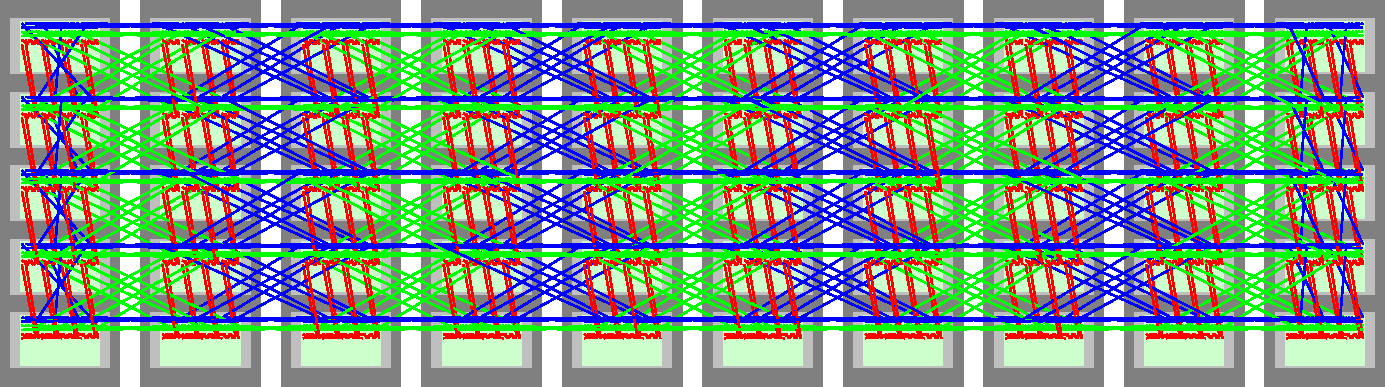
\includegraphics[width=\textwidth]{figures/spinnaker106}
				\caption[SpiNNaker machine mapped into cabinets and racks.]{The largest
				SpiNNaker machine with 1,200 boards and 1,036,800 cores mapped into 10
				cabinets of 5 racks each.  Coloured lines represent wires connecting
				{\color{red}North/South}, {\color{green}North-East/South-West} and
				{\color{blue}East/West} links.}
				\label{fig:spinnaker106}
			\end{figure}
			
			Even though the system is physically around six metres long, the longest
			wire will be less than one metre in length and thus within the S-ATA
			specification.
		
		\subsection{Future Work}
			
			% The tool has been successfuly used to
			% assemble machines (pictures!) and provide orders for cabling for the
			% next machines. Next stage will involve extending this to interactively
			% guiding larger builds and 
			
			TODO
	
	
	\section{Small-world networks}
		
		% Small world networks are: ... Allow lots of short paths, this means low
		% latency, low power and less contention. We describe ways of augmenting the
		% SpiNNaker network, making use of spare connections and resource for
		% board-to-board links while taking advantage of the physical arrangement
		% described in the previous section.
		
		Small-world networks are graphs with a very large number of nodes but,
		within which, the maximum shortest-path between pairs of nodes.
		Additionally, each node also features only a relatively small number of
		connections. They also contain `clusters' of well connected nodes, in
		contrast with random graphs (which may also fulfil the first criterion).
		
		Small world networks are often found in nature, perhaps most famously in
		social networks. In this context, the phenomenon was first observed in 1929
		by Hungarian author Frigyes Karinthy\cite{karinthy29} and has become
		popularly known by the name `six degrees of separation'. The theory states
		that for any two people on earth, chosen at random, there is a chain of at
		most 6 acquaintances which connects them.
		
		This property of maintaining low maximum shortest-path length while still
		remaining locally well connected is desirable for certain computational
		problems. In neural simulations, most communication is local with just a few
		longer connections. The clustering property of small world networks means
		these local connections can be well catered for while the low maximum
		shortest-path length means longer connections are still quick for very large
		models.
		
		In this section a simple method for constructing small-world networks is
		introduced which does require physically long connections while still
		exhibiting significant reductions in network latency.
		
		\subsection{Constructing small-world networks}
			
			% Add random links and lo-and-behold, smallworldness!
			
			Watts and Strogatz have proposed an algorithm for randomly constructing
			networks with small-world properties \cite{watts98}. The algorithm begins
			by creating a ring network with each node connecting to a fixed number of
			its neighbours (figure \ref{fig:ringNetworkB0}). In the next step, with a
			probability of $\beta$, each edge may be replaced by a random connection.
			For $0 < \beta < 1$, the networks produced exhibit varying degrees of the
			small-world properties (figure \ref{fig:ringNetworkB02}).  Finally, in the
			extreme case where $\beta=1$, the network devolves into a random network
			(figure \ref{fig:ringNetworkB1}).
			
			\begin{figure}
				\center
				\begin{subfigure}[t]{0.3\textwidth}
					\center
					\begin{tikzpicture}[thick,inner sep=0.1cm]
	\foreach \t in {30,60,...,360}{
		\node [fill,circle] at (\t:2) {};
		\draw (\t:2) -- (\t+30:2);
		\draw (\t:2) -- (\t+60:2);
	}
\end{tikzpicture}


					\caption{Ring ($\beta = 0.0$)}
					\label{fig:ringNetworkB0}
				\end{subfigure}
				\begin{subfigure}[t]{0.3\textwidth}
					\center
					\newcommand{\mayberandompath}[2]{
	\pgfmathsetmacro{\choice}{random(5)}
	\pgfmathsetmacro{\myrand}{random(12)*30}
	\ifthenelse{\equal{\choice}{1.0}}{
		\draw (#1:2) -- (#2+\myrand:2);
	}{
		\draw (#1:2) -- (#2:2);
	}
}

\begin{tikzpicture}[thick,inner sep=0.1cm]
	\foreach \t in {30,60,...,360}{
		\node [fill,circle] at (\t:2) {};
		\mayberandompath{\t}{\t+30}
		\mayberandompath{\t}{\t+60}
	}
\end{tikzpicture}

					\caption{Watts-Strogatz ($\beta = 0.2$)}
					\label{fig:ringNetworkB02}
				\end{subfigure}
				\begin{subfigure}[t]{0.3\textwidth}
					\center
					\newcommand{\mayberandompath}[2]{
	\pgfmathsetmacro{\myrand}{random(12)*30}
	\draw (#1:2) -- (#2+\myrand:2);
}

\begin{tikzpicture}[thick,inner sep=0.1cm]
	\foreach \t in {30,60,...,360}{
		\node [fill,circle] at (\t:2) {};
		\mayberandompath{\t}{\t+30}
		\mayberandompath{\t}{\t+60}
	}
	
\end{tikzpicture}

					\caption{Random ($\beta = 1.0$)}
					\label{fig:ringNetworkB1}
				\end{subfigure}
				
				\caption{Watts-Strogatz networks with a range of rewiring
				probabilities.}
				\label{fig:ringNetwork}
			\end{figure}
		
		\subsection{Modelling and results}
			
			% Don't need too many links to get a good return in terms of reduced
			% path length. Limiting results to short wires doesn't hurt too much,
			% especially after folding.
			
			This algorithm is readily extended to torus topologies similar to
			SpiNNaker's. In this preliminary work, a $k$-ary 2-cube (a two dimensional
			torus $k$ nodes long in each dimension) was used as the initial network as
			in figure \ref{fig:torusNetworkB0}.  Random permutations are introduced as
			in the Watts-Strogatz model resulting in a network such as figure
			\ref{fig:torusNetworkB01}.
			
			\begin{figure}
				\center
				\begin{subfigure}[t]{0.45\textwidth}
					\center
					\begin{tikzpicture}[thick,inner sep=0.1cm]
	\clip (-0.5,-0.5) rectangle (5.5,5.5);
	
	\node [fill,circle] (node 146024940) at (0,0) {};
	\node [fill,circle] (node 152407084) at (1,0) {};
	\node [fill,circle] (node 152406988) at (2,0) {};
	\node [fill,circle] (node 152407180) at (3,0) {};
	\node [fill,circle] (node 152407276) at (4,0) {};
	\node [fill,circle] (node 152407404) at (5,0) {};
	\node [fill,circle] (node 152407564) at (0,1) {};
	\node [fill,circle] (node 152407692) at (1,1) {};
	\node [fill,circle] (node 152407724) at (2,1) {};
	\node [fill,circle] (node 152407788) at (3,1) {};
	\node [fill,circle] (node 152407820) at (4,1) {};
	\node [fill,circle] (node 152407948) at (5,1) {};
	\node [fill,circle] (node 152531052) at (0,2) {};
	\node [fill,circle] (node 152531148) at (1,2) {};
	\node [fill,circle] (node 152531180) at (2,2) {};
	\node [fill,circle] (node 152531212) at (3,2) {};
	\node [fill,circle] (node 152531276) at (4,2) {};
	\node [fill,circle] (node 152537548) at (5,2) {};
	\node [fill,circle] (node 152553292) at (0,3) {};
	\node [fill,circle] (node 152553836) at (1,3) {};
	\node [fill,circle] (node 152554092) at (2,3) {};
	\node [fill,circle] (node 152554668) at (3,3) {};
	\node [fill,circle] (node 152554892) at (4,3) {};
	\node [fill,circle] (node 152580172) at (5,3) {};
	\node [fill,circle] (node 152580940) at (0,4) {};
	\node [fill,circle] (node 152581804) at (1,4) {};
	\node [fill,circle] (node 152610924) at (2,4) {};
	\node [fill,circle] (node 152609420) at (3,4) {};
	\node [fill,circle] (node 152656748) at (4,4) {};
	\node [fill,circle] (node 152656844) at (5,4) {};
	\node [fill,circle] (node 152656972) at (0,5) {};
	\node [fill,circle] (node 152657068) at (1,5) {};
	\node [fill,circle] (node 152657100) at (2,5) {};
	\node [fill,circle] (node 152657132) at (3,5) {};
	\node [fill,circle] (node 152657164) at (4,5) {};
	\node [fill,circle] (node 152657260) at (5,5) {};
	
	\draw (node 146024940)
							         .. controls +(0.500000,-1.000000)
							                 and +(0.500000,1.000000)
							         .. (node 152656972);
	\draw (node 146024940)
							         .. controls +(-1.000000,0.500000)
							                 and +(1.000000,0.500000)
							         .. (node 152407404);
	\draw (node 146024940) -- (node 152407084);
	\draw (node 146024940) -- (node 152407564);
	\draw (node 152407084) -- (node 152407692);
	\draw (node 152407084)
							         .. controls +(0.500000,-1.000000)
							                 and +(0.500000,1.000000)
							         .. (node 152657068);
	\draw (node 152406988) -- (node 152407180);
	\draw (node 152406988) -- (node 152407724);
	\draw (node 152406988) -- (node 152407084);
	\draw (node 152406988)
							         .. controls +(0.500000,-1.000000)
							                 and +(0.500000,1.000000)
							         .. (node 152657100);
	\draw (node 152407180)
							         .. controls +(0.500000,-1.000000)
							                 and +(0.500000,1.000000)
							         .. (node 152657132);
	\draw (node 152407180) -- (node 152407276);
	\draw (node 152407180) -- (node 152407788);
	\draw (node 152407276) -- (node 152407404);
	\draw (node 152407276) -- (node 152407820);
	\draw (node 152407276)
							         .. controls +(0.500000,-1.000000)
							                 and +(0.500000,1.000000)
							         .. (node 152657164);
	\draw (node 152407404) -- (node 152407948);
	\draw (node 152407404)
							         .. controls +(0.500000,-1.000000)
							                 and +(0.500000,1.000000)
							         .. (node 152657260);
	\draw (node 152407564)
							         .. controls +(-1.000000,0.500000)
							                 and +(1.000000,0.500000)
							         .. (node 152407948);
	\draw (node 152407564) -- (node 152531052);
	\draw (node 152407564) -- (node 152407692);
	\draw (node 152407692) -- (node 152407724);
	\draw (node 152407692) -- (node 152531148);
	\draw (node 152407724) -- (node 152407788);
	\draw (node 152407724) -- (node 152531180);
	\draw (node 152407788) -- (node 152407820);
	\draw (node 152407788) -- (node 152531212);
	\draw (node 152407820) -- (node 152531276);
	\draw (node 152407820) -- (node 152407948);
	\draw (node 152407948) -- (node 152537548);
	\draw (node 152531052) -- (node 152553292);
	\draw (node 152531052)
							         .. controls +(-1.000000,0.500000)
							                 and +(1.000000,0.500000)
							         .. (node 152537548);
	\draw (node 152531052) -- (node 152531148);
	\draw (node 152531148) -- (node 152553836);
	\draw (node 152531148) -- (node 152531180);
	\draw (node 152531180) -- (node 152554092);
	\draw (node 152531180) -- (node 152531212);
	\draw (node 152531212) -- (node 152531276);
	\draw (node 152531212) -- (node 152554668);
	\draw (node 152531276) -- (node 152537548);
	\draw (node 152531276) -- (node 152554892);
	\draw (node 152537548) -- (node 152580172);
	\draw (node 152553292) -- (node 152580940);
	\draw (node 152553292)
							         .. controls +(-1.000000,0.500000)
							                 and +(1.000000,0.500000)
							         .. (node 152580172);
	\draw (node 152553292) -- (node 152553836);
	\draw (node 152553836) -- (node 152554092);
	\draw (node 152553836) -- (node 152581804);
	\draw (node 152554092) -- (node 152610924);
	\draw (node 152554092) -- (node 152554668);
	\draw (node 152554668) -- (node 152554892);
	\draw (node 152554668) -- (node 152609420);
	\draw (node 152554892) -- (node 152580172);
	\draw (node 152554892) -- (node 152656748);
	\draw (node 152580172) -- (node 152656844);
	\draw (node 152580940)
							         .. controls +(-1.000000,0.500000)
							                 and +(1.000000,0.500000)
							         .. (node 152656844);
	\draw (node 152580940) -- (node 152656972);
	\draw (node 152580940) -- (node 152581804);
	\draw (node 152581804) -- (node 152610924);
	\draw (node 152581804) -- (node 152657068);
	\draw (node 152610924) -- (node 152657100);
	\draw (node 152609420) -- (node 152656748);
	\draw (node 152609420) -- (node 152610924);
	\draw (node 152609420) -- (node 152657132);
	\draw (node 152656748) -- (node 152656844);
	\draw (node 152656748) -- (node 152657164);
	\draw (node 152656844) -- (node 152657260);
	\draw (node 152656972)
							         .. controls +(-1.000000,0.500000)
							                 and +(1.000000,0.500000)
							         .. (node 152657260);
	\draw (node 152656972) -- (node 152657068);
	\draw (node 152657068) -- (node 152657100);
	\draw (node 152657100) -- (node 152657132);
	\draw (node 152657132) -- (node 152657164);
	\draw (node 152657164) -- (node 152657260);
\end{tikzpicture}

					\caption{Unmodified torus ($\beta=0.0$)}
					\label{fig:torusNetworkB0}
				\end{subfigure}
				\begin{subfigure}[t]{0.45\textwidth}
					\center
					\begin{tikzpicture}[thick,inner sep=0.1cm]
	\clip (-0.5,-0.5) rectangle (5.5,5.5);
	
	\node [fill,circle] (node 163015180) at (0,0) {};
	\node [fill,circle] (node 169393228) at (1,0) {};
	\node [fill,circle] (node 169393132) at (2,0) {};
	\node [fill,circle] (node 169393324) at (3,0) {};
	\node [fill,circle] (node 169393420) at (4,0) {};
	\node [fill,circle] (node 169393548) at (5,0) {};
	\node [fill,circle] (node 169393708) at (0,1) {};
	\node [fill,circle] (node 169393836) at (1,1) {};
	\node [fill,circle] (node 169393868) at (2,1) {};
	\node [fill,circle] (node 169393932) at (3,1) {};
	\node [fill,circle] (node 169393964) at (4,1) {};
	\node [fill,circle] (node 169394092) at (5,1) {};
	\node [fill,circle] (node 169521292) at (0,2) {};
	\node [fill,circle] (node 169521388) at (1,2) {};
	\node [fill,circle] (node 169521420) at (2,2) {};
	\node [fill,circle] (node 169521452) at (3,2) {};
	\node [fill,circle] (node 169521516) at (4,2) {};
	\node [fill,circle] (node 169527788) at (5,2) {};
	\node [fill,circle] (node 169543532) at (0,3) {};
	\node [fill,circle] (node 169544076) at (1,3) {};
	\node [fill,circle] (node 169544332) at (2,3) {};
	\node [fill,circle] (node 169544908) at (3,3) {};
	\node [fill,circle] (node 169545132) at (4,3) {};
	\node [fill,circle] (node 169574508) at (5,3) {};
	\node [fill,circle] (node 169575276) at (0,4) {};
	\node [fill,circle] (node 169576140) at (1,4) {};
	\node [fill,circle] (node 169601164) at (2,4) {};
	\node [fill,circle] (node 169599660) at (3,4) {};
	\node [fill,circle] (node 169646988) at (4,4) {};
	\node [fill,circle] (node 169647084) at (5,4) {};
	\node [fill,circle] (node 169647212) at (0,5) {};
	\node [fill,circle] (node 169647308) at (1,5) {};
	\node [fill,circle] (node 169647340) at (2,5) {};
	\node [fill,circle] (node 169647372) at (3,5) {};
	\node [fill,circle] (node 169647404) at (4,5) {};
	\node [fill,circle] (node 169647500) at (5,5) {};
	
	\draw (node 163015180) -- (node 169393228);
	\draw (node 163015180)
							         .. controls +(-1.000000,0.500000)
							                 and +(1.000000,0.500000)
							         .. (node 169393548);
	\draw (node 163015180)
							         .. controls +(0.500000,-1.000000)
							                 and +(0.500000,1.000000)
							         .. (node 169575276);
	\draw (node 163015180)
							         .. controls +(0.500000,-1.000000)
							                 and +(0.500000,1.000000)
							         .. (node 169647212);
	\draw (node 169393228) -- (node 169647500);
	\draw (node 169393228) -- (node 169393836);
	\draw (node 169393228)
							         .. controls +(0.500000,-1.000000)
							                 and +(0.500000,1.000000)
							         .. (node 169647308);
	\draw (node 169393132) -- (node 169393324);
	\draw (node 169393132) -- (node 169393228);
	\draw (node 169393132)
							         .. controls +(0.500000,-1.000000)
							                 and +(0.500000,1.000000)
							         .. (node 169647340);
	\draw (node 169393132) -- (node 169393868);
	\draw (node 169393324)
							         .. controls +(0.500000,-1.000000)
							                 and +(0.500000,1.000000)
							         .. (node 169647372);
	\draw (node 169393324) -- (node 169393420);
	\draw (node 169393324) -- (node 169393932);
	\draw (node 169393420) -- (node 169393548);
	\draw (node 169393420)
							         .. controls +(0.500000,-1.000000)
							                 and +(0.500000,1.000000)
							         .. (node 169521516);
	\draw (node 169393420) -- (node 169393964);
	\draw (node 169393548)
							         .. controls +(0.500000,-1.000000)
							                 and +(0.500000,1.000000)
							         .. (node 169647500);
	\draw (node 169393548) -- (node 169394092);
	\draw (node 169393708)
							         .. controls +(-1.000000,0.500000)
							                 and +(1.000000,0.500000)
							         .. (node 169394092);
	\draw (node 169393708) -- (node 169521292);
	\draw (node 169393708) -- (node 169393836);
	\draw (node 169393836) -- (node 169393868);
	\draw (node 169393836) -- (node 169521388);
	\draw (node 169393836) -- (node 169647340);
	\draw (node 169393868) -- (node 169393932);
	\draw (node 169393932) -- (node 169647212);
	\draw (node 169393932) -- (node 169543532);
	\draw (node 169393932) -- (node 169521452);
	\draw (node 169393932) -- (node 169521516);
	\draw (node 169393964) -- (node 169394092);
	\draw (node 169394092) -- (node 169527788);
	\draw (node 169394092)
							         .. controls +(0.500000,-1.000000)
							                 and +(0.500000,1.000000)
							         .. (node 169647500);
	\draw (node 169521292)
							         .. controls +(-1.000000,0.500000)
							                 and +(1.000000,0.500000)
							         .. (node 169527788);
	\draw (node 169521292) -- (node 169543532);
	\draw (node 169521292) -- (node 169521388);
	\draw (node 169521420) -- (node 169521452);
	\draw (node 169521420) -- (node 169544332);
	\draw (node 169521452) -- (node 169544908);
	\draw (node 169521452) -- (node 169521516);
	\draw (node 169521516) -- (node 169527788);
	\draw (node 169521516) -- (node 169647340);
	\draw (node 169521516) -- (node 169545132);
	\draw (node 169527788) -- (node 169574508);
	\draw (node 169543532) -- (node 169544076);
	\draw (node 169543532) -- (node 169575276);
	\draw (node 169544076) -- (node 169544332);
	\draw (node 169544076) -- (node 169576140);
	\draw (node 169544332) -- (node 169544908);
	\draw (node 169544332) -- (node 169601164);
	\draw (node 169544908) -- (node 169545132);
	\draw (node 169544908) -- (node 169599660);
	\draw (node 169545132) -- (node 169574508);
	\draw (node 169545132) -- (node 169646988);
	\draw (node 169574508) -- (node 169647084);
	\draw (node 169575276)
							         .. controls +(-1.000000,0.500000)
							                 and +(1.000000,0.500000)
							         .. (node 169647084);
	\draw (node 169575276) -- (node 169647212);
	\draw (node 169576140) -- (node 169601164);
	\draw (node 169576140) -- (node 169647308);
	\draw (node 169601164) -- (node 169647340);
	\draw (node 169599660) -- (node 169646988);
	\draw (node 169599660) -- (node 169601164);
	\draw (node 169599660) -- (node 169647372);
	\draw (node 169646988) -- (node 169647084);
	\draw (node 169646988) -- (node 169647404);
	\draw (node 169647212)
							         .. controls +(-1.000000,0.500000)
							                 and +(1.000000,0.500000)
							         .. (node 169647500);
	\draw (node 169647212) -- (node 169647308);
	\draw (node 169647308) -- (node 169647340);
	\draw (node 169647372) -- (node 169647404);
	
\end{tikzpicture}

					\caption{Rewired torus ($\beta=0.1$)}
					\label{fig:torusNetworkB01}
				\end{subfigure}
				
				\caption{Extension of the Watts-Strogatz model to a 6-ary 2-cube.}
				\label{fig:torusNetwork}
			\end{figure}
			
			A $k$-ary $n$-cube has an average shortest path length of $\frac{nk}{4}$.
			This is because a packet travels (on average, under uniform random
			traffic) $\frac{1}{4}$ of the way around each of the $n$, $k$-node-long
			dimensions. In this case, that means the average path length is $\frac{2
			\times 6}{4} = 3$.
			
			\begin{figure}
				\center
				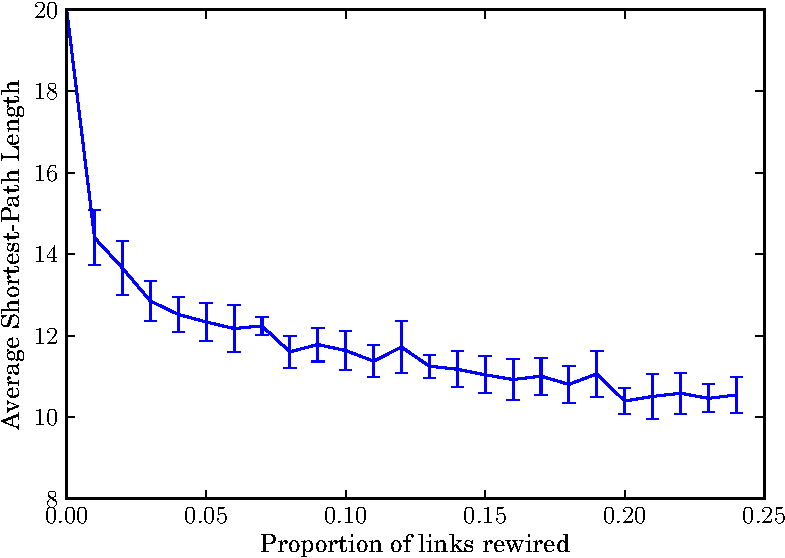
\includegraphics[width=0.7\textwidth]{figures/smallWorldTorus}
				\caption[Average shortest-path length for folded 40-ary 2-cube.]{Average
				shortest-path length for folded 40-ary 2-cube (mean of 10 runs, error
				bars show 1 standard deviation).}
				\label{fig:smallWorldTorus}
			\end{figure}
			
			Experiments using a simple graph-based model were carried out to determine
			the effects of rewiring on shortest-path length.  For the randomly rewired
			rewired network shown, the average shortest path is now reduced from 3 to
			2.77 hops.  Further, this model was used to confirm findings by Shin et
			al.  \cite{shin11} who found an increase in bandwidth (though the findings
			also apply to latency) when even just a small number of links are rewired
			as shown in figure \ref{fig:smallWorldTorus}.
			
			Unfortunately, by na\"ively adding random links it is possible for
			long-distance connections to be introduced into the network. As described
			in the previous section, these physically long connections can cause
			problems for electrical high-speed serial links.
			
			Though techniques exist to attempt to optimally lay-out networks
			containing random wiring \cite{koibuchi13}, these do not deal well with
			networks which also feature a large degree of regularity. An alternative
			approach is to simply limit the length of wires randomly inserted.
			Though this fails to yield large reductions in path length in examples
			laid out na\"ively as in figure \ref{fig:torusNetwork}, if the network is
			folded (as described in the previous section), significant reductions can
			be achieved.
			
			\begin{figure}
				\center
				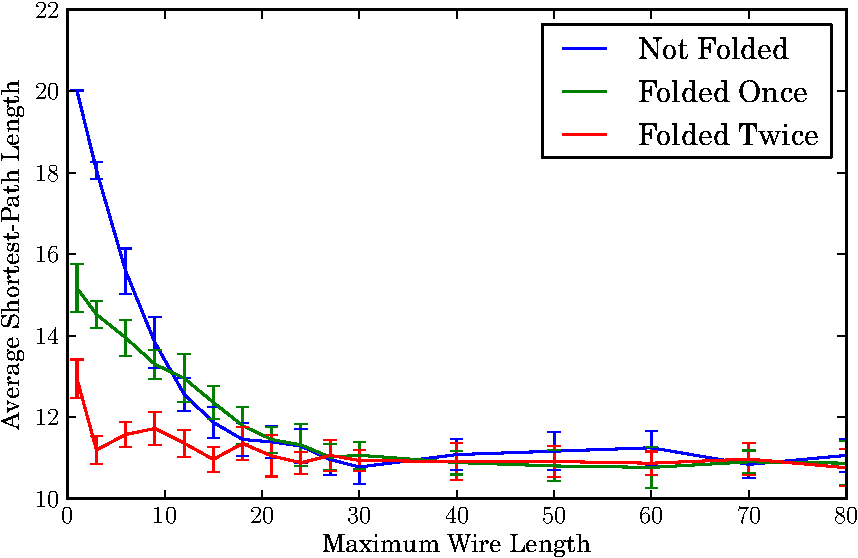
\includegraphics[width=0.7\textwidth]{figures/smallWorldLimitedWiring}
				\caption{Average shortest-path length for folded 40-ary 2-cube with 1\%
				rewiring}
				\label{fig:smallWorldLimitedWiring}
			\end{figure}
			
			Figure \ref{fig:smallWorldLimitedWiring} shows the effect of rewiring 1\%
			of links when the maximum length of a randomly inserted wire is limited.
			For networks folded twice (as in the case of the proposed SpiNNaker wiring
			plan), limiting wire length has little impact.
		
		\subsection{Further work}
			
			Figure \ref{fig:ringNetworkLimitedWires} shows valid random links in a
			small ring network with limited wire lengths. Nodes near the top and
			bottom of the ring potentially have shorter average path lengths compared
			with other nodes than nodes near the left and right of the ring. This is
			because the allowed links for top and bottom nodes connect nodes greater
			logical distances apart in the ring than those allowed on the left and
			right. The result is that the average path length from two different nodes
			becomes non-uniform across nodes in different parts of the system.
			
			\begin{figure}
				\center
				\begin{tikzpicture}[thick,inner sep=0.1cm]
	\foreach [count=\n] \t in {30,60,...,360}{
		\draw [help lines] (\t:2) -- (\t+30:2);
	}
	\foreach [count=\n] \t in {30,60,...,360}{
		\node [fill,circle] at (90-\t:2) (node \n) {};
	}
	
	\draw (node 8) to (node 10);
	\draw (node 8) to (node 11);
	
	\draw (node 7) to (node 11);
	\draw (node 7) to (node 12);
	
	\draw (node 6) to (node 12);
	\draw (node 6) to (node 1);
	
	\draw (node 5) to (node 1);
	\draw (node 5) to (node 2);
	
	\draw (node 4) to (node 2);
	
\end{tikzpicture}


				\caption[Valid random links in a folded ring network with short
				wires.]{Valid random links in ring network when wires limited to a
				length of 1 unit and the network is folded as in figure
				\ref{fig:folding}.}
				\label{fig:ringNetworkLimitedWires}
			\end{figure}
			
			The effect of this non-uniformity is yet to be studied. In addition, the
			magnitude of the differences in average path length in different parts of
			a network is reduced both in higher dimensional topologies and also after
			the network has been folded and mapped into physical racks and cabinets.
			Future work intends to implement a small-world style network both within
			the simulator described in the next section and, subsequently, within
			SpiNNaker's board-to-board links.
	
	
	\section{SpiNNaker network modelling}
		
		% Colaboration with others researching simulator platforms, due for journal
		% submission in coming months, final stages of writing. Context of the work:
		% want to try out modelling on different platforms. My contribution: some
		% writing and the development of an accurate software simulator for
		% SpiNNaker's interconnect. This work indirectly offers interesting insights
		% into behaviours due to the board-to-board links.
		
		A recent collaboration with other researchers within the department has
		investigated novel methods for high-level simulation and modelling of large
		scale systems. This work used SpiNNaker's interconnection network as its
		case study and included the development of a number of different simulators
		including both software and FPGA-based models. The work revealed that modern
		high-level languages for FPGA and hardware development such as Bluespec
		System Verilog (BSV) \cite{nikhil04} have reached a level of development
		efficiency comparable with software. This result demonstrates that modellers
		are no-longer faced with a decision of whether time allows for a hardware
		model but rather whether advantages of FPGA-based models such as substantial
		simulation speed improvements are desired over software based approaches.
		The work is in its final draft and targeted for journal submission early in
		August this year.
		
		The author's primary contribution to this work has centred around the
		development of a detailed software model of SpiNNaker's interconnection
		network. In addition, a significant portion of the analysis of the
		simulators was also carried out. In this section, the simulator, named
		`Tickysim', is described below along with brief summary of results
		demonstrating faithfulness to the system it models. The section concludes
		with plans to use this simulator to guide future research.
		
		\subsection{Software simulator model}
			
			% Model 18 cores as traffic generators/consumers. Links are modelled as
			% delay elements (accurately captures req/ack links), internal arbitration
			% scheme is modelled along with pipelined router.
			
			\begin{figure}
				\begin{subfigure}[b]{0.65\textwidth}
					\center
					\tikzexternaldisable
					\begin{tikzpicture}[thick,remember picture,font=\small]
	
	\def\arbwidth{0.3cm}
	\def\arbheight{0.7cm}
	\def\arboffset{0.15cm}
	
	% An arbiter. Arguments:
	% 1: Name
	% 2: Node args
	% 3: Draw style
	\newcommand{\arb}[3]{
		\node (#1)
		      [minimum width=\arbwidth,minimum height=\arbheight, inner sep=0,#2]
		      {}
		      ;
		
		\coordinate (#1 in 1) at ($(#1.south west)!0.75!(#1.north west)$);
		\coordinate (#1 in 2) at ($(#1.south west)!0.25!(#1.north west)$);
		\coordinate (#1 out)  at (#1.east);
		
		\draw [#3]
		      (#1.south west)
		   -- (#1.north west)
		   -- ([yshift=-\arboffset]#1.north east)
		   -- ([yshift=\arboffset]#1.south east)
		   -- cycle
		      ;
	}
	
	% A buffer. Arguments:
	% 1: Name
	% 2: Node args
	% 3: Draw style
	% 4: Number of slots x
	% 5: Number of slots y
	\newcommand{\buf}[5]{
		\pgfmathsetlengthmacro{\bufsize}{0.2cm}
		\pgfmathsetlengthmacro{\width}{sqrt(#4)*\bufsize}
		\pgfmathsetlengthmacro{\height}{sqrt(#5)*\bufsize}
		\node (#1)
		      [ draw
		      , minimum width=\width
		      , minimum height=\height
		      , inner sep=0
		      , #2
		      , #3
		      ] { };
		
		% Draw Lines on buffers to indicate number of slots
		\foreach \x in {1,...,#4}{
			\ifthenelse{\not\equal{\x}{#4}}{
				\pgfmathsetmacro{\xx}{\x/#4}
				\draw [#3] ($(#1.south west)!\xx!(#1.south east)$)
				        -- ($(#1.north west)!\xx!(#1.north east)$);
			}{}
		}
		\foreach \y in {1,...,#5}{
			\ifthenelse{\not\equal{\y}{#5}}{
				\pgfmathsetmacro{\yy}{\y/#5}
				\draw [#3] ($(#1.south west)!\yy!(#1.north west)$)
				        -- ($(#1.south east)!\yy!(#1.north east)$);
			}{}
		}
		
		\coordinate (#1 in)  at (#1.west);
		\coordinate (#1 out) at (#1.east);
	}
	
	% A buffer-arbiter pair. Arguments:
	% 1: Name
	% 2: Arbiter node args
	% 3: Draw style
	% 4: Number of buffer slots x
	% 5: Number of buffer slots y
	\newcommand{\arbbuf}[5]{
		\arb{#1 arb}{#2}{#3}
		\buf{#1 buf}{right=\arbbufgap of #1 arb}{#3}{#4}{#5}
		\draw [#3] (#1 arb out) -- (#1 buf in);
	}
	
	% Draw a line with two bends. Arguments:
	% 1: Start
	% 2: End
	% 3: Draw style
	% 4: Bend 1 style
	% 5: Bend 2 style
	\newcommand{\drawbent}[5]{
		\draw [#3] (#1) #4 ($(#1)!0.5!(#2)$) #5 (#2);
	}
	
	\def\arbbufgap{0.1cm}
	\def\arbvgap{0.1cm}
	\def\arbhgap{0.4cm}
	
	\def\routerhgap{0.5cm}
	
	% Output Buffers. Arguments:
	% 1: Output name
	% 2: Line first bend y offset
	% 3: Line first bend x offset
	\newcommand{\outbuf}[3]{
		\path let \p1=(#1 buf in), \p2=([xshift=0.5*\routerhgap]router.east) in (\x2,\y1) coordinate (#1 out);
		\buf{#1 out buf}{right=\routerhgap of #1 out}{}{2}{1}
		\draw ($(router.north east)!#2!(router.south east)$)
		   -- ++(#3,0)
		   |- (#1 out buf)
		      ;
	}
	
	\def\packetgenvgap{0.6cm}
	
	% The node itself
	\node (model) [draw, rectangle, inner sep=0.25cm] {
		\begin{tikzpicture}[thick,remember picture]
			% Level 2
			\arbbuf{e ne}{}{}{1}{1}
			\buf{e  buf}{left=\arbbufgap of e ne arb in 1}{}{2}{1} \draw (e  buf) -- (e ne arb in 1);
			\buf{ne buf}{left=\arbbufgap of e ne arb in 2}{}{2}{1} \draw (ne buf) -- (e ne arb in 2);
			
			\arbbuf{n w}{below=\arbvgap of  e ne arb}{}{1}{1}
			\buf{n buf}{left=\arbbufgap of n w arb in 1}{}{2}{1} \draw (n buf) -- (n w arb in 1);
			\buf{w buf}{left=\arbbufgap of n w arb in 2}{}{2}{1} \draw (w buf) -- (n w arb in 2);
			\arbbuf{sw s}{below=\arbvgap of n w arb}{}{1}{1}
			\buf{sw buf}{left=\arbbufgap of sw s arb in 1}{}{2}{1} \draw (sw buf) -- (sw s arb in 1);
			\buf{s  buf}{left=\arbbufgap of sw s arb in 2}{}{2}{1} \draw (s  buf) -- (sw s arb in 2);
			\arbbuf{proc}{below=\arbvgap of sw s arb}{draw=white}{1}{1}
			
			% Level 1
			\arbbuf{e ne n w}{right=\arbhgap of $(e ne buf)!0.5!(n w buf)$}{}{1}{1}
			\drawbent{e ne buf out}{e ne n w arb in 1}{}{-|}{|-}
			\drawbent{n w buf out}{e ne n w arb in 2}{}{-|}{|-}
			\arbbuf{sw s proc}{right=\arbhgap of $(sw s buf)!0.5!(proc buf)$}{}{1}{1}
			\drawbent{sw s buf out}{sw s proc arb in 1}{}{-|}{|-}
			\coordinate (proc in) at  (sw s proc arb in 2);
			
			% Level 0 (root)
			\arbbuf{root}{right=\arbhgap of $(e ne n w buf)!0.5!(sw s proc buf)$}{}{2}{1}
			\drawbent{e ne n w buf out}{root arb in 1}{}{-|}{|-}
			\drawbent{sw s proc buf out}{root arb in 2}{}{-|}{|-}
			
			% Router
			\def\routerstages{4}
			\node (router)
			      [inner ysep=0.5cm,inner xsep=1em,draw, rectangle, right=\arbbufgap of root buf out]
			      {Router}
			      ;
			\draw (root buf out) -- (router.west);
			
			% Router pipeline stage divisions
			\begin{scope}
				\clip       ($(router.south west)!0.0!(router.north west)$)
				  rectangle ($(router.south east)!0.2!(router.north east)$)
				            ($(router.south west)!0.8!(router.north west)$)
				  rectangle ($(router.south east)!1.0!(router.north east)$)
				  ;
				
				\foreach \x in {2,...,\routerstages}{
					\pgfmathsetmacro{\xx}{(\x-1)/\routerstages}
					\draw  ($(router.south west)!\xx!(router.south east)$)
					    -- ($(router.north west)!\xx!(router.north east)$);
				}
			\end{scope}
			
			\outbuf{e}{ 0.2}{0.3*\routerhgap + 0.1cm}
			\outbuf{ne}{0.3}{0.3*\routerhgap + 0.2cm}
			\outbuf{n}{ 0.4}{0.3*\routerhgap + 0.3cm}
			\outbuf{w}{ 0.5}{0.3*\routerhgap + 0.4cm}
			\outbuf{sw}{0.6}{0.3*\routerhgap + 0.3cm}
			\outbuf{s}{ 0.7}{0.3*\routerhgap + 0.2cm}
			
			% Packet Generator
			\node (packet gen)
			      [below=\packetgenvgap of sw s proc arb in 2, xshift=-0.5*\arbhgap]
			      [draw, rectangle, text width = 2cm, align=center, inner sep=0.2cm]
			      {Packet Generator}
			    ;
			
			\buf{packet gen buf}{above=\arbbufgap of packet gen.north}{}{1}{2}
			\draw (packet gen buf.north) |- (sw s proc arb in 2);
			\draw (packet gen.north) -- (packet gen buf.south);
			
			% Packet Consumer
			\path let \p1=(router.south)
			        , \p2=(packet gen.north)
			      in coordinate (packet con north) at (\x1,\y2);
			\node (packet con)
			      [below=0 of packet con north,xshift=0.7cm]
			      [draw, rectangle, text width = 2cm, align=center, inner sep=0.2cm]
			      {Packet Consumer}
			    ;
			\draw ($(router.north east)!0.8!(router.south east)$)
			   -- ++(0.3*\routerhgap + 0.1cm, 0)
			      coordinate (packet con router output)
			    ;
			\path let \p1=(packet con router output)
			        , \p2=(packet con.north)
			      in coordinate (packet con input) at (\x1,\y2);
			\buf{packet con buf}{above=\arbbufgap of packet con input}{}{1}{2}
			\draw (packet con input) -- (packet con buf.south);
			\draw (packet con router output) -- (packet con buf.north);
			
		\end{tikzpicture}
	};
	
	
	\def\keyentrygap{1.5em}
	\def\keylabelgap{0.3cm}
	
	% The Key
	\node [below=0.5cm of model, inner sep=0] {
		\begin{tikzpicture}[thick,remember picture]
			
			\arb{key arb}{}{}
			\node (key arb label) [right=\keylabelgap of key arb] {Round-Robin Arbiter};
			
			\buf{key buf}{right=\keyentrygap of key arb label}{}{1}{1}
			\node (key buf label) [right=\keylabelgap of key buf] {Buffer};
			
			\node [left=\keyentrygap of key arb] {Key:};
		\end{tikzpicture}
	};
	
	
	\def\inpindist{0.75cm}
	\def\outpindist{0.8cm}
	
	% XXX: Note that the text here differs from the labelling used internally.
	% This is due to the fact that the original assignment was discovered to be
	% erroneuous and just correcting the text was easier than replacing
	% everything.
	
	% Input pins
	\draw (e  buf in) -- ++(-\inpindist,0) node [left] {E};
	\draw (ne buf in) -- ++(-\inpindist,0) node [left] {S};
	\draw (n  buf in) -- ++(-\inpindist,0) node [left] {NE};
	\draw (w  buf in) -- ++(-\inpindist,0) node [left] {N};
	\draw (sw buf in) -- ++(-\inpindist,0) node [left] {W};
	\draw (s  buf in) -- ++(-\inpindist,0) node [left] {SW};
	
	% Output pins
	\draw (e  out buf out) -- ++(\outpindist,0) node [right] {E};
	\draw (ne out buf out) -- ++(\outpindist,0) node [right] {S};
	\draw (n  out buf out) -- ++(\outpindist,0) node [right] {NE};
	\draw (w  out buf out) -- ++(\outpindist,0) node [right] {N};
	\draw (sw out buf out) -- ++(\outpindist,0) node [right] {W};
	\draw (s  out buf out) -- ++(\outpindist,0) node [right] {SW};
	
\end{tikzpicture}

					\caption{Model of a SpiNNaker chip. A packet
					generator and consumer models SpiNNaker's eighteen cores. A tree of
					packet arbiters mimmicing SpiNNaker's Network on Chip (NoC) feeds a
					stream of packets into a router model.}
					\label{fig:tickysim-model-chip}
				\end{subfigure}
				~~~~~
				\begin{subfigure}[b]{0.28\textwidth}
					\centering
					% A diagram showing links delays between nodes.
\begin{tikzpicture}[thick,font=\small]
	
	\def\nodesize{1.0cm}
	\def\scale{2.1}
	
	\begin{scope}[scale=\scale]
		\clip (-0.85,-0.85) rectangle ( 0.85, 0.85);
		
		\foreach \x in {-1,...,1}{
			\foreach \y in {-1,...,1}{
				\node [ draw
				      , rectangle
				      , minimum width=\nodesize
				      , minimum height=\nodesize
				      , inner sep=0
				      ]
				      (node \x\y)
				      at (\x,\y)
				      {};
			}
		}
	\end{scope}
	
	\newcommand{\link}[2]{
		\draw (#1) to (#2);
		\node [ draw
		      , fill=white
		      , rectangle
		      , inner sep=0.1cm
		      ]
		      at ($(#1)!0.5!(#2)$)
		      {D};
	}
	
	% Links from the central node outward
	\foreach \x/\y in {1/0, 0/1, 1/1, -1/0, 0/-1, -1/-1}{
		\link{node 00}{node \x\y}
	}
	% Other visible links (not the central node)
	\link{node 0-1}{node 10}
	\link{node -10}{node 01}
	
\end{tikzpicture}

					\vspace{1.8cm}
					
					\caption{Delay elements inserted between chips model the effects of
					link latency.}
					\label{fig:tickysim-model-link-delays}
				\end{subfigure}
				
				\caption{The Tickysim simulator model.}
				\label{fig:tickysim-model}
			\end{figure}
			
			The basic unit of the Tickysim simulator model is a high-level of a single
			SpiNNaker chip which is summarised in figure
			\ref{fig:tickysim-model-chip}.
			
			Since the model focuses on the interconnection network, the eighteen
			processors present on a SpiNNaker chip are instead modelled by a simple
			packet generator and consumer. This simplification saves a large amount of
			simulation overhead at the expense of detail in processor behaviour. Since
			this is not the focus of the model, this simplification should
			significantly impact results.
			
			The model captures the basic structure of the Network-on-Chip (NoC) within
			SpiNNaker chips. In particular, streams of packets incident on the chip
			are merged using a tree structure before entering the on-chip router. The
			simulated router models a multiple stage pipeline matching that of the
			actual SpiNNaker router.
			
			The complete model consists of a network of chips interconnected by delay
			elements as illustrated in figure \ref{fig:tickysim-model-link-delays}.
			These delay elements model the latency encountered by packets crossing a
			chip-to-chip boundary.
			
			The model is extensively instrumented and configurable to allow a range of
			metrics to be collected and numerous parameters such as buffer sizes,
			injected traffic patterns and router behaviour to be modified. In
			addition, the software architecture is structured to allow straightforward
			extension making it suitable for use in later work.
			
			When configured to model a 144-chip SpiNNaker system, the model runs
			around 7,000 times slower than real time on an Intel Xeon E3-1225 V2
			running at 3.2 GHz and 32 GB of RAM, the same order of magnitude slow-down
			experienced by comparable software simulators such as INSEE
			\cite{navaridas11insee}. Though the model itself is single threaded,
			parameter-sweep style experiments may be performed in parallel using
			commodity compute resources. In practice, experiments were conducted using
			idle department workstations allowing hundreds of parameter settings to be
			simultaneously simulated in the time taken to run a single simulation on a
			single machine.
		
		\subsection{Results}
			
			% Experiments performed showed highly matched behaviour between the model
			% and SpiNNaker but reveal the effects of the non-homogeneity introduced
			% by board-to-board links for certain traffic patterns.
			
			Experiments were carried out to verify that the simulators bore a close
			resemblance to the actual SpiNNaker hardware. These consisted of injecting
			a suite of synthetic traffic patterns at various injection rates and
			monitoring standard metrics such as number of packets dropped and accepted
			load (number of packets arriving at their destination).
			
			\begin{figure}
				\begin{subfigure}{\textwidth}
					% Commands for producing plots as used in the paper.

% Plot an accepted/dropped packet load graph
% Arguments:
%  #1: Number of nodes in the system
%  #2: Traffic pattern name
\newcommand{\plotresults}[2]{%
	\begin{tikzpicture}
		\newcommand{\width}{0.48\textwidth}
		\newcommand{\height}{5.5cm}
		
		%\selectcolormodel{gray};
		
		\begin{axis}[ xlabel=Injection Rate
		            , ylabel=Accepted Load
		            , xmin=0, xmax=1
		            , ymin=0
		            , width=\width
		            , height=\height
		            , yticklabel style = { /pgf/number format/precision=1
		                                 , /pgf/number format/fixed
		                                 , /pgf/number format/fixed zerofill
		                                 }
		            ]
			\addplot+ table [x=injection_rate, y=accepted_load] {results/#1_spinnaker_#2.csv};
			\addplot+ table [x=injection_rate, y=accepted_load] {results/#1_tickysim_#2.csv};
		\end{axis}
		
		\begin{axis}[ xshift=\width+0.2cm
		            , xlabel=Injection Rate
		            , ylabel=Dropped Packets
		            , xmin=0, xmax=1
		            , ymin=0
		            , width=\width
		            , height=\height
		            %, yticklabel pos=right
		            , yticklabel style = { /pgf/number format/precision=1
		                                 , /pgf/number format/fixed
		                                 , /pgf/number format/fixed zerofill
		                                 }
		            , legend pos=south east
		            , legend entries = { SpiNNaker
		                               , Tickysim
		                               }
		            ]
			\addplot+ table [x=injection_rate, y=dropped] {results/#1_spinnaker_#2.csv};
			\addplot+ table [x=injection_rate, y=dropped] {results/#1_tickysim_#2.csv};
		\end{axis}
	\end{tikzpicture}%
}

					\plotresults{144}{cyclic}
					
					\caption{`Uniform' traffic.}
					\label{fig:results-144-accuracy-cyclic}
				\end{subfigure}
				
				\vspace{1em}
				
				\begin{subfigure}{\textwidth}
					% Commands for producing plots as used in the paper.

% Plot an accepted/dropped packet load graph
% Arguments:
%  #1: Number of nodes in the system
%  #2: Traffic pattern name
\newcommand{\plotresults}[2]{%
	\begin{tikzpicture}
		\newcommand{\width}{0.48\textwidth}
		\newcommand{\height}{5.5cm}
		
		%\selectcolormodel{gray};
		
		\begin{axis}[ xlabel=Injection Rate
		            , ylabel=Accepted Load
		            , xmin=0, xmax=1
		            , ymin=0
		            , width=\width
		            , height=\height
		            , yticklabel style = { /pgf/number format/precision=1
		                                 , /pgf/number format/fixed
		                                 , /pgf/number format/fixed zerofill
		                                 }
		            ]
			\addplot+ table [x=injection_rate, y=accepted_load] {results/#1_spinnaker_#2.csv};
			\addplot+ table [x=injection_rate, y=accepted_load] {results/#1_tickysim_#2.csv};
		\end{axis}
		
		\begin{axis}[ xshift=\width+0.2cm
		            , xlabel=Injection Rate
		            , ylabel=Dropped Packets
		            , xmin=0, xmax=1
		            , ymin=0
		            , width=\width
		            , height=\height
		            %, yticklabel pos=right
		            , yticklabel style = { /pgf/number format/precision=1
		                                 , /pgf/number format/fixed
		                                 , /pgf/number format/fixed zerofill
		                                 }
		            , legend pos=south east
		            , legend entries = { SpiNNaker
		                               , Tickysim
		                               }
		            ]
			\addplot+ table [x=injection_rate, y=dropped] {results/#1_spinnaker_#2.csv};
			\addplot+ table [x=injection_rate, y=dropped] {results/#1_tickysim_#2.csv};
		\end{axis}
	\end{tikzpicture}%
}

					\plotresults{144}{complement}
					
					\caption{`Complement' traffic.}
					\label{fig:results-144-accuracy-complement}
				\end{subfigure}
				
				\caption[Packet acceptance and dropping in SpiNNaker
				and TIckysim.]{Comparison of packet acceptance and dropping rates in
				SpiNNaker and TIckysim. Values scaled such that 1.0 represents the
				maximum rate at which packets may pass through a chip-to-chip link.}
				\label{fig:results-144-accuracy}
			\end{figure}
			
			Figure \ref{fig:results-144-accuracy-cyclic} gives a representative
			example of the majority results obtained. In this example, a `uniform'
			traffic pattern was used where nodes produce traffic destined for each
			node in the system in turn. Both SpiNNaker and the Tickysim model exhibit
			classic behaviour for this pattern with all traffic being accepted until
			the network saturates.  Beyond saturation, packets are dropped. Since
			packets are dropped after a fixed timeout, this increases the time between
			sending of packets and thus causes the accepted load to drop to a fixed
			low.
			
			\begin{figure}
				\center
				% Comparison of three heatmaps of SpiNNaker's complement traffic pattern.
\begin{tikzpicture}[baseline]
	% Produce a single heatmap for comparison of the SpiNNaker complement traffic
	% pattern.
	% Arguments:
	%  #1: The injection rate
	%  #2: Extra arguments for the axis environment
	%  #3: Title
	\newcommand{\spinncomplementheatmap}[3]{
		\begin{axis}[ xlabel=X
		            , title={#3}
		            , title style={align=center}
		            , axis equal=true
		            , colorbar style={ ylabel={Packets Dropped}
		                             , yticklabel pos = left
		                             , yticklabel style = { /pgf/number format/precision=3
		                                                  , /pgf/number format/fixed
		                                                  , /pgf/number format/fixed zerofill
		                                                  }
		                             }
		            , colormap={blackwhite}{rgb=(0,0,0); rgb=(1,1,1)}
		            , view={0}{90}
		            , xmin=-0.5, xmax=11.5
		            , ymin=-0.5, ymax=11.5
		            , point meta min=0, point meta max=0.018
		            , xtick={0,3,...,11}
		            , ytick={0,3,...,11}
		            , minor tick num=2
		            , #2
		            ]
			\addplot3 [ surf
			          , shader=flat corner
			          ] table [ x expr={\thisrow{chip_x}-0.5}
			                  , y expr={\thisrow{chip_y}-0.5}
			                  , z expr={\thisrow{dumped} / 1200000}
			                  ] {results/SpiNNaker_complement_#1.csv}
			          ;
			\addplot+ [ no markers
			          , gray
			          , ultra thick
			          ] table {results/threeboard_outline.csv}
			          ;
		\end{axis}
	}
	
	\newcommand{\stdwidth}{0.27\textwidth}
	\newcommand{\stdoffset}{(\stdwidth-0.50cm)}
	
	\spinncomplementheatmap{0.10}{ width = \stdwidth
	                             , height = \stdwidth
	                             , xshift=0*\stdoffset
	                             , ylabel=Y
	                             }{Before saturation}
	\spinncomplementheatmap{0.30}{ width = \stdwidth
	                             , height = \stdwidth
	                             , xshift=1*\stdoffset
	                             , yticklabel={$ $}
	                             }{Semi-saturated}
	\spinncomplementheatmap{0.40}{ width = \stdwidth
	                             , height = \stdwidth
	                             , xshift=2*\stdoffset
	                             , yticklabel={$ $}
	                             , colorbar
	                             , colorbar style={xshift=1.3cm}
	                             }{Fully saturated}
\end{tikzpicture}

				\caption[Packet dropping in a three board SpiNNaker machine.]{Packet
				dropping in a three board SpiNNaker machine under complement traffic at
				various injection rates. Thick lines show boundaries between boards in
				the system.}
				\label{fig:heatmap-spinnaker-complement}
			\end{figure}
			
			Some traffic patterns such as `complement', however, exhibited artefacts
			in SpiNNaker due to the prototype implementation of the HSS links between
			boards not being able to achieve full bandwidth. Since the difference due
			to these links is not modelled by Tickysim, their results clearly differ.
			Figure \ref{fig:results-144-accuracy-complement} demonstrates this effect
			in the form of two distinct phases of saturation in SpiNNaker but just one
			in Tickysim. In this pattern, distinct clusters of communicating nodes
			occur in the network. In SpiNNaker, those clusters crossing board
			boundaries saturate first due to their lower bandwidth followed later by
			the native chip-to-chip links causing the two phases as shown in figure
			\ref{fig:heatmap-spinnaker-complement}.
		
		\subsection{Further work}
			
			% Plans to include models of SpiNNaker links. Preliminary trials at
			% accurately modelling these have been unsuccessful. Will be used to guide
			% work on these links.
			
			Work is planned to more accurately model the behaviour of board-to-board
			links within Tickysim to allow its use in evaluating the utility of small
			world connectivity. Preliminary, simplistic attempts to model
			board-to-board links as simply having longer latencies have been
			unsuccessful. It is suspected that the mechanisms used within the HSS
			links are the underlying root of the problem.
	
	
	\section{SpiNNaker FPGA connectivity}
		
		% Work started at CapoCaccia with input from various parties to get
		% SpiNNaker peripherals working. The start of a project to get peripherals
		% properly integrated and generally add some routing smarts to the FPGAs
		
		At the 2014 Capo Caccia Neuromorphic Workshop requirements for extending the
		HSS links available within SpiNNaker for connecting peripherals and to host
		computers for the purposes of loading neural models and extracting results.
		As a result of these discussions, work began to extend the existing
		infrastructure used for board-to-board links to support flexible additional
		connectivity. This work has concentrated on the development of FPGA designs
		to support tasks such as routing packets to and from peripherals and hosts
		and the integration of HSS links operating at different speeds.
		
		This section outlines the existing infrastructure followed by a description
		of the extensions developed and how they address the requirements proposed
		at the workshop. The section concludes with planned future work which builds
		on the infrastructure developed.
		
			\subsection{Existing infrastructure}
				
				% Description of what exists already in the board-to-board links,
				% outline the protocol's principles. Also describe the rdy/vld
				% interface.
				
				\begin{figure}
					\center
					\begin{tikzpicture}[thick]
	\def\twoofsevenheight{1.0em}
	\def\twoofsevensep{1.5em}
	
	\def\bordersep{1.0em}
	
	% 2-of-7 link handlers
	\foreach \row in {0,...,7}{
		\node [ draw
		      , rectangle
		      , yshift=\row*\twoofsevensep
		      , inner sep=0.3em
		      , minimum height=\twoofsevenheight
		      ]
		      (two of seven \row)
		      {\tiny{2 of 7}};
	}
	
	% Framing block
	\node [ draw
	      , rectangle
	      , right=of $(two of seven 0.east)!0.5!(two of seven 7.east)$
	      , minimum height = 7*\twoofsevensep + \twoofsevenheight
	      , text width=2.5cm
	      , align=center
	      ]
	      (framing)
	      {Framing and Reliability};

	% Links from 2-of-7 to framing
	\foreach \row in {0,...,7}{
		\draw [<->]
		      (two of seven \row.east)
		   -- (two of seven \row.east -| framing.west)
		    ;
	}
	
	% Links from 2-of-7 to chips
	\foreach \row in {0,...,7}{
		\draw [<->]
		      (two of seven \row.west)
		   -- ++(-1cm,0) coordinate (two of seven wire \row)
		    ;
	}
	
	% GTP
	\node [ draw
	      , rectangle
	      , right=of framing
	      , minimum height = 7*\twoofsevensep + \twoofsevenheight
	      , text width=2.5cm
	      , align=center
	      ]
	      (gtp)
	      {Gigabit Transceiver\\(Hard IP)};
	
	% Framing to/from GTP wires
	\draw [<->] (framing.east) -- (gtp.west);
	
	% Gigabit links
	\draw [<->] (gtp.east) -- ++(1cm,0) coordinate (gtp wire);
	
	% FPGA Border
	\draw ([shift={(-\bordersep,-\bordersep)}]two of seven 0.south west)
	      rectangle
	      ([shift={( \bordersep, \bordersep)}]gtp.north east);
	
	% Chip label
	\node [ left=0 of $(two of seven wire 0)!0.5!(two of seven wire 7)$
	      , rotate=90
	      , anchor=south
	      ]
	      {SpiNNaker Chip Links};
	
	% HSS link label
	\node [ right=0 of gtp wire
	      , rotate=90
	      , anchor=north
	      ]
	      {S-ATA connector};
\end{tikzpicture}

					
					\caption[Existing board-to-board link FPGA design.]{Existing
					board-to-board link FPGA design. Each FPGA contains two independent
					copies of this design so that the three FPGAs on each board can
					implement all six board-to-board links.}
					\label{fig:existing-fpga-links}
				\end{figure}
				
				The existing board-to-board links are implemented within the FPGAs on
				SpiNNaker boards. Each HSS link is designed to transparently replace
				eight chip-to-chip SpiNNaker links. The design, as shown in figure
				\ref{fig:existing-fpga-links} contains three basic elements. A 2-of-7
				block translates between the asynchronous 2-of-7 protocol used by
				SpiNNaker chip links and a synchronous protocol used within the FPGA
				design. The next block assembles and disassembles `frames' containing
				SpiNNaker packets and ensures reliable communication by verifying
				incoming frames and retransmitting frames if required. The final block
				is provided as `hard IP' rather than soft programmable FPGA logic and
				serialises and deserialises frames over the HSS link.
				
				\begin{figure}
					\center
					\begin{tikzpicture}[thick]
						\input{|"wavedromtikz.py wavedrom figures/rdyvld-protocol.drom"}
					\end{tikzpicture}
					
					\caption{Example of the ready/valid protocol.}
					\label{fig:rdyvld-protocol}
				\end{figure}
				
				Within and between blocks, data is transferred using a simple
				point-to-point `ready/valid' protocol illustrated in figure
				\ref{fig:rdyvld-protocol}.  The receiever asserts a `ready' signal
				whenever it is able to accept new data. The sender places data it wishes
				to send on a data bus while asserting a `valid' signal. If the valid and
				ready signals are simultaneously asserted on the next rising edge of the
				clock, the data is considered received. This protocol allows a value to
				be transmitted up-to every clock cycle while allowing both the sender
				and receiver control over the rate that data flows.
			
			\subsection{Proof-of-concept I/O device}
				
				% Describe principle of how a router will be integrated and streams
				% merged.
				
				To allow extension of the existing board-to-board system, the
				ready/valid protocol described above, with the databus being the width
				of a long SpiNNaker packet (70 bits) has been standardised for
				communication between new blocks.
				
				\begin{figure}
					\center
					\begin{tikzpicture}[thick]
	\def\twoofsevenheight{1.0em}
	\def\twoofsevensep{1.5em}
	
	\def\bordersep{1.0em}
	
	% Router
	\node [ draw
	      , rectangle
	      , anchor=north west
	      , minimum height = 1cm + 7*\twoofsevensep + \twoofsevenheight
	      , text width=1.5cm
	      , align=center
	      ]
	      (router)
	      {Router};
	
	% Framing blocks
	\node [ draw
	      , rectangle
	      , right=of router.north east
	      , anchor = north west
	      , minimum height = 3.5*\twoofsevensep + 0.5*\twoofsevenheight
	      , text width=2.5cm
	      , align=center
	      ]
	      (framing)
	      {Framing and Reliability};
	\node [ draw
	      , rectangle
	      , below=of framing
	      , minimum height = 3.5*\twoofsevensep + 0.5*\twoofsevenheight
	      , text width=2.5cm
	      , align=center
	      ]
	      (framing periph)
	      {Framing and Reliability};
	
	% 2-of-7 link handlers
	\foreach \row [count=\i from 0] in {-3.5,...,3.5}{
		\node [ draw
		      , rectangle
		      , yshift=\row*\twoofsevensep
		      , inner sep=0.3em
		      , minimum height=\twoofsevenheight
		      , left= of router.west
		      ]
		      (two of seven \i)
		      {\tiny{2 of 7}};
	}

	% Links from 2-of-7 to router
	\foreach \row in {0,...,7}{
		\draw [<->]
		      (two of seven \row.east)
		   -- (two of seven \row.east -| router.west)
		    ;
	}

	% Links from router to b2b framing
	\foreach \row in {-3.5,...,3.5}{
		\draw [<->]
		      ([yshift=-0.7em*\row]framing.west -| router.east)
		   -- ([yshift=-0.7em*\row]framing.west)
		    ;
	}
	
	% Links from router to periph framing
	\foreach \row in {-3.5,...,3.5}{
		\draw [<->]
		      ([yshift=-0.7em*\row]framing periph.west -| router.east)
		   -- ([yshift=-0.7em*\row]framing periph.west)
		    ;
	}
	
	% Links from 2-of-7 to chips
	\foreach \row in {0,...,7}{
		\draw [<->]
		      (two of seven \row.west)
		   -- ++(-1cm,0) coordinate (two of seven wire \row)
		    ;
	}
	
	% GTPs
	\node [ draw
	      , rectangle
	      , right=of framing
	      , minimum height = 3.5*\twoofsevensep + 0.5*\twoofsevenheight
	      , text width=2.5cm
	      , align=center
	      ]
	      (gtp)
	      {Gigabit Transceiver\\(Hard IP)};
	\node [ draw
	      , rectangle
	      , below=of gtp
	      , minimum height = 3.5*\twoofsevensep + 0.5*\twoofsevenheight
	      , text width=2.5cm
	      , align=center
	      ]
	      (gtp periph)
	      {Gigabit Transceiver\\(Hard IP)};
	
	% Framing to/from GTP wires
	\draw [<->] (framing.east)        -- (gtp.west);
	\draw [<->] (framing periph.east) -- (gtp periph.west);
	
	% Gigabit links
	\draw [<->] (gtp.east)        -- ++(1cm,0) coordinate (gtp wire);
	
	% FPGA Border
	\draw ([shift={(-\bordersep, \bordersep)}]router.north -| two of seven 7.west)
	      rectangle
	      ([shift={( \bordersep,-\bordersep)}]gtp periph.south east);
	
	% Chip label
	\node [ left=0 of $(two of seven wire 0)!0.5!(two of seven wire 7)$
	      , rotate=90
	      , anchor=south
	      ]
	      (spinnaker chip links label)
	      {SpiNNaker Chip Links};
	
	% HSS link label
	\node [ right=0 of gtp wire
	      , rotate=90
	      , anchor=north
	      ]
	      {Board-to-Board};
	
	
	%%%%%%%%%%%%%%%%%%%%%%%%%%%%%%%%%%%%%%%%%%%%%%%%%%%%%%%%%%%%%%%%%%%%%%%%%%%%%%%%
	% Peripheral
	%%%%%%%%%%%%%%%%%%%%%%%%%%%%%%%%%%%%%%%%%%%%%%%%%%%%%%%%%%%%%%%%%%%%%%%%%%%%%%%%
	
	
	% Framing block
	\node [ draw
	      , rectangle
	      , below=1.5cm of framing periph
	      , minimum height = 3.5*\twoofsevensep + 0.5*\twoofsevenheight
	      , text width=2.5cm
	      , align=center
	      ]
	      (framing device)
	      {Framing and Reliability};
	
	% UART block
	\node [ draw
	      , rectangle
	      , left = of framing device.south west
	      , anchor = south east
	      , minimum height = 1.8em
	      , text width=1.5cm
	      , align=center
	      ]
	      (uart)
	      {UART};
	
	
	% Links from UART to b2b framing
	\foreach \row in {-3.5,...,2.5}{
		\draw [<->]
		      ([yshift=-0.7em*\row]framing device.west)
		   -- ++(-0.5cm,0)
		      node [xshift=-0.5ex] {$\times$}
		    ;
	}
	\draw [<->]
	      ([yshift=-0.7em*3.5]framing device.west)
	   -- ([yshift=-0.7em*3.5]uart.east |- framing device.west)
	    ;
	
	% GTP
	\node [ draw
	      , rectangle
	      , below=1.5cm of gtp periph
	      , minimum height = 3.5*\twoofsevensep + 0.5*\twoofsevenheight
	      , text width=2.5cm
	      , align=center
	      ]
	      (gtp device)
	      {Gigabit Transceiver\\(Hard IP)};
	
	% Framing to/from GTP wires
	\draw [<->] (framing device.east) -- (gtp device.west);
	
	% Gigabit links
	\draw [<->]
	      (gtp periph.east)
	   -- ++(1cm,0)
	   |- (gtp device.east);
	
	% FPGA Border
	\draw ([shift={(-\bordersep, \bordersep)}]uart.west |- framing device.north)
	      rectangle
	      ([shift={( \bordersep,-\bordersep)}]gtp device.south east);
	
	% Link to USB
	\draw [<->] (uart.west) -- ++(-1cm,0) coordinate (uart connection);
	
	\node [left=0 of uart connection] {Host PC};
	
	
	
	
	\draw [decorate,decoration={brace,amplitude=1em,raise=1ex}]
	      ([shift={(0,-\bordersep)}]spinnaker chip links label.north |- router.south)
	   -- coordinate (spinnaker label)
	      ([shift={(0, \bordersep)}]spinnaker chip links label.north |- router.north);
	
	\draw [decorate,decoration={brace,amplitude=1em,raise=1ex}]
	      ([shift={(0,-\bordersep)}]spinnaker chip links label.north |- uart.south)
	   -- coordinate (periph label)
	      ([shift={(0, \bordersep)}]spinnaker chip links label.north |- framing device.north);
	
	\node [left=1.5em of spinnaker label, rotate=90, anchor=south] {SpiNNaker FPGA};
	\node [left=1.5em of periph label, rotate=90, anchor=south] {Raggedstone 2};
	
	
\end{tikzpicture}

					
					\caption[Proof-of-concept low-speed I/O system.]{Proof-of-concept
					low-speed I/O system. A spare HSS link from an FPGA on a SpiNNaker
					board connects to a Raggedstone 2 board connected to a host PC.}
					\label{fig:proof-of-concept-fpga-links}
				\end{figure}
				
				Based on the ready/valid standard, a number of basic components for
				extending the existing design were produced. Using these components, a
				simple proof of concept low-speed host connection was developed and is
				sketched in figure \ref{fig:proof-of-concept-fpga-links}. In this
				system, A SpiNNaker board is connected to an off-the-shelf Raggedstone 2
				FPGA development baord \cite{raggedstone2} using a spare S-ATA
				connector. A host PC then connects to the Raggedstone 2 via an onboard
				FTDI USB-to-UART (Universal Asynchronous Receiver/Transmitter) converter
				providing a simple to drive, low speed (2.3 Mbit/s) connection over
				which SpiNNaker packets can be transmitted.
				
				A router is added to the SpiNNaker FPGA design which is able to route a
				stream of packets from the incoming SpiNNaker chips either along their
				usual board-to-board connection or to the Raggedstone 2 board, or both.
				Packets are routed using the same key and mask mechanism used within a
				SpiNNaker chip, though only one key and mask is available, rather than
				1,024. Packets routed to the Raggedstone 2 board are transmitted via the
				same HSS link protocol as board-to-board links.
				
				On the Raggedstone 2 board, one of the eight streams of packets is fed
				to a UART block which uses a simple protocol to send and receive
				SpiNNaker packets at low speed to a host PC. The UART connection of the
				host is the bottleneck in the system, the router within the SpiNNaker
				FPGAs introduces 13 ns of additional latency but with no throughput
				cost.
				
				This proof-of-concept device has been successfully integrated into the
				SpiNNaker implementation of Nengo where it can be used to transmit
				values in and out of a model in real time. Despite its low bandwidth,
				the link carries raw SpiNNaker packets with no protocol overheads and
				actually performs favourably compared to the current Ethernet
				implementation in SpiNNaker's Nengo implementation which suffers
				extremely large protocol overheads.
			
			\subsection{Further work}
				
				% Next steps will involve getting basic routing up and running, then on
				% to my planned project, see next chapter.
				
				With the basic infrastructure in place for implementing custom routing
				schemes and using additional HSS links within SpiNNaker's FPGAs in
				place, it is now possible to use this to develop high speed peripheral
				and host connectivity. In addition, this infrastructure allows for the
				addition of axillary links between boards allowing the implementation of
				small-world network connectivity.
				
				In collaboration with researchers at the Technical University of Munich,
				a small board containing an FPGA with both a HSS link and a USB 3.0 link
				is being developed. This board's FPGA could be loaded with a design very
				similar to that developed for the Raggedstone 2 but with the UART block
				replaced with a USB 3.0 block. Using this board, it is hoped that very
				high bandwidth communication between a host and SpiNNaker machine should
				become possible.


	\chapter{Research plan}
	\label{sec:research-plan}
	
	% Generally planning to massage the existing system to make better use of
	% serial links, looking at powering down strategies and testing things both in
	% simulation (using existing simulator) and also using real traffic in
	% SpiNNaker. To this end I will be continuing background activities involving
	% working with neural modelling.
	
	\begin{figure}
		\center
		\begin{tikzpicture}[thick,x=0.25cm]

%%%%%%%%%%%%%%%%%%%%%%%%%%%%%%%%%%%%%%%%%%%%%%%%%%%%%%%%%%%%%%%%%%%%%%%%%%%%%%%%
% Hacked-up Gantt Library
%%%%%%%%%%%%%%%%%%%%%%%%%%%%%%%%%%%%%%%%%%%%%%%%%%%%%%%%%%%%%%%%%%%%%%%%%%%%%%%%

% An entry in the Gantt chart. Takes a label, start offset, length and slack.
% Also defines a pair of labels "[label] start" and "[label] end" which can be
% used for drawing dependency lines.
\newcommand{\ganttEntry}[4]{
	% Label
	\node (label)
				[below=1.5ex of label.south east,anchor=east,minimum height=1.7em]
				{#1}
				;
	\coordinate (gantt labels end) at (label.south east);
	
	% Box
	\draw [fill=white]
	      ([shift={(#2   ,-.9ex)}]label.north east) rectangle
	      ([shift={(#2+#3,0.9ex)}]label.south east);
	
	% The tips of the box
	\coordinate (#1 end)
	         at ([shift={(#2+#3,0.9ex)}]label.south east);
	\coordinate (#1 start)
	         at ([shift={(#2   ,-.9ex)}]label.north east);
	
	% Slack line
	\draw [ultra thick]
	      ([shift={(#2+#3,0)}]$(label.north east)!0.5!(label.south east)$)
	   -- ++(#4,0);
}

\newcommand{\ganttDep}[2]{
	\draw [->,red] (#1 end) -| (#2 start);
}

\newcommand{\ganttVSep}[2]{
	\draw [#2] ([shift={(#1,0)}]gantt labels start) -- ([shift={(#1,0)}]gantt labels end);
}

% A new gantt chart. Takes a list of x-offset/label/major-label tuples. For each
% tuple a line is created with x-offset from the previous line and the span is
% labelled with "label". If major-label given, a major label will be drawn
% centered over the previous entries up until the last major-label.
\newenvironment{gantt}[1]{
	% Start the list of labels
	\node (label) [white] {Ag};
	\coordinate (gantt labels start) at (label.north east);
	\def\periods{#1}
}{
	\begin{scope}[on background layer]
		% Thick line separating from labels
		\draw (gantt labels start) -- (gantt labels end);
		
		% Start of the area covered by a "major" label
		\coordinate (gantt maj label start) at (gantt labels start);
		
		\foreach \x/\lab/\mlab in \periods {
			\coordinate (next gantt labels start) at ([shift={(\x,0)}]gantt labels start);
			\coordinate (next gantt labels end)   at ([shift={(\x,0)}]gantt labels end);
			
			% Minor label
			\node at ($(gantt labels start) !0.5! (next gantt labels start)$)
			      [anchor=west,rotate=90]
			      {\lab}
			      ;
			
			% Separator
			\ifthenelse{\equal{\mlab}{}}{
				\draw [help lines] (next gantt labels start) -- (next gantt labels end);
			}{
				\draw [help lines,thick] (next gantt labels start) -- (next gantt labels end);
			}
			
			\coordinate (gantt labels start) at (next gantt labels start);
			\coordinate (gantt labels end)   at (next gantt labels end);
			
			% Major label
			\ifthenelse{\equal{\mlab}{}}{}{
				\coordinate (next gantt maj label start) at (gantt labels start);
				\node at ($(gantt maj label start) !0.5! (next gantt maj label start)$)
				      [yshift=1cm,anchor=south]
				      {\mlab}
				      ;
				\coordinate (gantt maj label start) at (next gantt maj label start);
			}
		}
	\end{scope}
}



%%%%%%%%%%%%%%%%%%%%%%%%%%%%%%%%%%%%%%%%%%%%%%%%%%%%%%%%%%%%%%%%%%%%%%%%%%%%%%%%
% The Chart...
%%%%%%%%%%%%%%%%%%%%%%%%%%%%%%%%%%%%%%%%%%%%%%%%%%%%%%%%%%%%%%%%%%%%%%%%%%%%%%%%

\begin{gantt}{
	4/Sep/, 4/Oct/, 4/Nov/, 4/Dec/2014,%
	3/Q1/, 3/Q2/, 3/Q3/, 3/Q4/2015,%
	3/Q1/, 3/Q2/2016%
}
	\ganttEntry{Nengo Network Experiments}       {0}{4}{8}
	\ganttEntry{Small-World Modelling}           {0}{4}{2}
	\ganttEntry{Small-World HSS Impelementation} {4}{8}{4}
	\ganttEntry{Small-World Benchmarking}        {10}{6}{1}
	\ganttEntry{USB 3.0 Interface}               {16}{2}{2}
	\ganttEntry{HSS Power Management}            {16}{5}{2}
	\ganttEntry{Power Management Benchmarking}   {21}{3}{1}
	
	\ganttEntry{Thesis Writing}     {24}{8}{2}
	
	\ganttDep{Small-World Modelling}{Small-World HSS Impelementation}
	\ganttDep{Nengo Network Experiments}{Small-World Benchmarking}
	\ganttDep{Small-World HSS Impelementation}{HSS Power Management}
	\ganttDep{HSS Power Management}{Power Management Benchmarking}
\end{gantt}

\end{tikzpicture}

		\caption[Gantt chart overview of research plan.]{Gantt chart overview of
		research plan. Boxes indicate expected duration of a task, thick lines
		indicate slack and red arrows show dependencies between tasks. Note the
		non-linear scale.}
		\label{fig:plan-gantt}
	\end{figure}
	
	The preliminary work so-far has focused on 
	
	\section{FPGA-based routing}
		
		% Develop routing scheme for SpiNNaker packets suitable for peripheral, host
		% and preliminary small-world communications via the SpiNNaker links. This
		% scheme will continue to make use of the current HSS protocol blocks.
		
		\subsection{Host communication}
			
			% Snooping, loading, etc.
		
		\subsection{Peripheral communication}
			
			% Configuration and hetrogenaity
		
		\subsection{Board-to-board communication}
			
			% Small world networks
	
	
	\section{SpiNNaker traffic analysis}
		
		% To better target efforts and gain further understanding, work with Mundrew
		% on Nengo network experiments to assess performance.  Must try to get a
		% picture of what demand for links will be like. High-speed links offer a
		% unique peek into network traffic beyond what is offered by existing
		% counters.
	
	\section{High-speed serial power control}
		
		% Work to try and make some power savings by powering down idle links or
		% reducing speed (to reduce link transitions), taking into account latency
		% concerns for SpiNNaker.
		
		\subsection{Power-down and bring-up}
			
			% Specify latency issues, describe current technologies for doing this and
			% appropriate signalling stuff. See PCI-E, S-ATA and friends.
		
		\subsection{Speed changing}
			
			% Possible application of link speeds being set in response to demand.
		
		\subsection{Always-on links}
			
			% Use a selection of always-on serial links when demand is low or others
			% are being powered up. How do small-world links fit in this picture?
		
		\subsection{`Santos-28' test chip}
			
			% A 28 nm test chip is being developed with TU Dresden to evaluate various
			% technologies' performance for inclusion in a second generation SpiNNaker
			% chip. There may be room in this space for my own involvement in this
			% work at short notice.
	
	
	\section{Performance evaluation}
		
		% Can build on work by Evangelos to see how performance in terms of power
		% works out with various FPGA based things going on. Hopefuly steal some of
		% his test networks. Can also sneak myself into work on SPAUN performance
		% messings.

	\chapter{Conclusion}
	
	% Brain is interesting but tough to deal with, existing machines struggle to
	% make the grade in terms of performance.
	%
	% Neuromorphic hardware offers the potential to scale up much more easily.
	% SpiNNaker is a fun example of a digital approach to this. It avoids problems
	% faced by existing systems.
	%
	% TODO: Finish-off.


	
	% Number bib entries by order of appearance
	\bibliographystyle{unsrt}
	\bibliography{report}
	
\end{document}
